\section{Case study: the 1955 automobile price war}\label{sec:06-bresnahan}

The vertical model entered empirical industrial organization through a study of conduct.
\citet{Bresnahan1987} asks whether the American automobile boom of 1955 was a price war. The paper embeds the
vertical model of \cref{sec:06-vertical} in an oligopoly model with multi-product firms. It solves the model under
two conduct hypotheses, collusion and Bertrand-Nash competition, and estimates each version by maximum likelihood
for the model years 1954, 1955 and 1956. Non-nested tests then ask which hypothesis the data favor in each year. No
cost data enter. Conduct is identified from the fine structure of the cross-section of products. What matters is
which products are close neighbors in quality, and whether a close neighbor belongs to the same firm or to a rival.

The section follows the order of a full case study. We state the question and the facts
(\cref{sec:06-bres-question,sec:06-bres-facts}), describe the data (\cref{sec:06-bres-data}), and set out the
model (\cref{sec:06-bres-model}). We then prove the equilibrium properties on which the test rests. Markups rise
whenever a pair of neighbors starts to cooperate, collusive markups have a closed form, and Bertrand markups of
close rivals vanish. Estimation, the non-nested test, the estimates, the counterfactual and the robustness checks
follow (\cref{sec:06-bres-estimation,sec:06-bres-cox,sec:06-bres-estimates,sec:06-bres-fit,sec:06-bres-robust}).
The section closes with identification, critiques and the contribution of the paper
(\cref{sec:06-bres-ident,sec:06-bres-limits,sec:06-bres-contribution}).

\subsection{The question and why it matters}\label{sec:06-bres-question}

In the 1955 model year, American passenger car production was about 45 percent higher than in the two
surrounding years, while quality-adjusted prices were lower \citep[p.~457]{Bresnahan1987}. Aggregate demand models
fit that year poorly. \citet[pp.~168--169]{Chow1960}, a leading study of automobile demand, reports that ``the
year 1955 is an exception'' to the rule of small residuals. Its 1955 residual is ``twice as large as the standard
error'' (quoted in \citealp[footnote~1]{Bresnahan1987}). Paul Samuelson stated the puzzle more
sharply. He ``would flunk any econometrics paper that claimed to provide an explanation of 1955 auto
sales.''\footnote{Bresnahan reports the classroom remark and attributes the anecdote to Robert E. Hall
\citep[footnote~2]{Bresnahan1987}.}

Higher output at a lower price is the signature of a supply shift. A pure demand shock moves the market along an
upward-sloping supply relation and raises price, so it cannot produce a price trough in a boom on its own.
Bresnahan therefore looks for a supply shock, and he proposes one of a specific form. His hypothesis is a one-year
breakdown of tacit collusion among the automakers. Under this hypothesis firms priced to maximize joint profits in
the 1954 and 1956 model years and competed in prices in the 1955 model year. The 1955 boom was then, in part, a
price war.

The paper matters for three reasons. First, it is the first structural test of conduct in a differentiated-products
industry, and it works without any data on costs. \citet[p.~844]{BerryLevinsohnPakes1995} call it ``perhaps the
first attempt at simultaneously modeling and estimating the demand and oligopoly pricing sides of the market.''
Conduct is encoded in a cooperation matrix $\Omega$, the same object that merger simulation changes when two firms
combine (\cref{ch:mergers}). Second, it shows that conduct can change over time within one industry. This links it
to the empirical study of collusion (\cref{ch:collusion-evidence}), where \citet{Porter1983} documents switches
between collusive and non-collusive periods in a railroad cartel from time-series data. Bresnahan instead uses the
cross-section of products within each year.

Third, a price war in a boom year speaks to theories of collusion over the business cycle
(\cref{ch:collusion-theory}). In \citet{RotembergSaloner1986}, collusion is hardest to sustain when current demand
is high relative to future demand, so collusive prices fall in booms. They read Bresnahan's results as support for
their theory, because 1955 was a boom year.\footnote{The 1984 NBER working-paper version of
\citet{RotembergSaloner1986} discusses Bresnahan's study in its section on evidence.} In
\citet{GreenPorter1984}, by contrast, price wars follow unexpectedly low demand. The 1955 episode fits the first
theory better. Bresnahan does not test either theory. His contribution is to show that the conduct of 1955 differed
from that of the neighboring years. He later judged that such evidence had not separated the theories, and he doubted that further studies of the
same kind would. Rotemberg and
Saloner combine the regime switches that \citet{Porter1983} reports with the pattern of conduct that
\citet{Bresnahan1987} finds. \citet[p.~1025]{Bresnahan1989} sees ``little in these investigations that
differentiates among the various theories.'' The timing of changes in conduct is harder to estimate than its
average level. A study of what starts and ends price wars has as many observations as there are price wars, far
fewer than the number of periods.

\subsection{Setting and aggregate facts}\label{sec:06-bres-facts}

The American industry of the mid-1950s consisted of three large firms, General Motors (GM), Ford and Chrysler, and
a fringe of smaller producers that included American Motors (AMC). Firms sell several models each. The time unit
is the \emph{model year}: the row labelled 1955 in the tables covers the fourth quarter of 1954 through the third
quarter of 1955. Bresnahan treats the model year as a short run in a precise sense. Within it, firms set prices and
quantities, but their product lines are predetermined. With fixed costs of product development, products are
imperfect substitutes in equilibrium. Even the ``competitive'' model therefore has market power. The label refers
to noncooperative conduct. Even competing firms are not price takers \citep[p.~458]{Bresnahan1987}.

\begin{table}[htbp]
\centering
\caption{Aggregate indicators of the automobile market, model years 1953--1957}
\label{tab:06-bres-facts}
\small
\begin{tabular}{@{}lrrrrr@{}}
\toprule
 & 1953 & 1954 & 1955 & 1956 & 1957 \\
\midrule
\multicolumn{6}{@{}l}{\textit{Automobile market (Bresnahan's Table I)}} \\
(1) Production, millions of units & 6.13 & 5.51 & 7.94 & 5.80 & 6.12 \\
(2) Real price: CPI for new cars relative to the CPI & 1.01 & 0.99 & 0.95 & 0.97 & 0.98 \\
(3) Quality-adjusted price (Cagan), percent change & NA & NA & $-2.5$ & 6.3 & 6.1 \\
(4) Real sales, billions of 1957 dollars & 14.5 & 13.9 & 18.4 & 15.7 & 16.2 \\
(5) Quantity index, (4) divided by (2), 1957 $=100$ & 86.8 & 84.9 & 117.2 & 97.9 & 100.0 \\
\addlinespace
\multicolumn{6}{@{}l}{\textit{Outside the automobile market (Bresnahan's Table II)}} \\
(6) Per capita disposable personal income & 1623 & 1609 & 1659 & 1717 & 1732 \\
(7) Three-month Treasury bill rate, percent & 1.9 & 0.9 & 1.7 & 2.6 & 3.2 \\
(8) Non-auto durables spending, billions of 1957 dollars & 14.5 & 14.5 & 16.1 & 17.1 & 17.0 \\
(9) Accounting profits of the automakers & 2.58 & 2.25 & 3.91 & 2.21 & 2.38 \\
\bottomrule
\end{tabular}

\smallskip
\begin{minipage}{0.95\textwidth}
\footnotesize
\emph{Notes:} Reproduced from \citet[Tables I and II, p.~459]{Bresnahan1987}. Rows are model years. Nominal values
are deflated with the GNP deflator. Row (3) is the percentage change in Cagan's (1971) quality-adjusted price
index, which uses only physically unchanged models. Row (4) is auto output in constant dollars from the National
Income and Product Accounts. The source's note for row (6) reads ``billions of 1957 dollars'', which cannot apply to
a per capita figure. The values are 1957 dollars per person. Row (9) is the profit of the five largest automobile
companies. The note that should give its units is not printed in the source.
\end{minipage}
\end{table}

\Cref{tab:06-bres-facts} shows why 1955 is anomalous. Production jumped to 7.94 million cars. This is 44 percent
above 1954, 37 percent above 1956, and 40.4 percent above the average of the two years. Bresnahan's round figure of
45 percent is close to the comparison with 1954. At the same time the real
price of new cars hit its trough of 0.95. Quality adjustment does not change the picture. The quality-adjusted index
of \citet{Cagan1971} fell by 2.5 percent in 1955 and rose by 6.3 percent in 1956. Bresnahan notes that the hedonic
index of \citet{Griliches1964} behaves similarly.

Row (4) adds a second fact. Real sales in value terms rose by 32 percent between 1954 and 1955, much less than the
44 percent rise in units. The implicit quantity index of row (5) rose by more than real sales. Bresnahan reads this
as a one-year shift of buyers toward smaller, lower-value cars, and he points to production by price group in
\emph{Ward's Automotive Yearbook} (his footnote~3). The shift matters later, because the price war hypothesis
predicts that competition intensifies most in the small-car segment.

Rows (6) to (8) show that demand factors explain part of the boom. Per capita income rose by 3.1 percent in 1955.
The Treasury bill rate of 1.7 percent was below its 1956 and 1957 levels. Spending on other durables rose by 11
percent in 1955, but it did not fall in 1956, while automobile output collapsed. Bresnahan concludes that some of
the 1955 increase was due to demand, but that a full demand-side explanation would ``need to be fairly fancy''
\citep[p.~460]{Bresnahan1987}.

Row (9) invites a wrong inference. Accounting profits jumped from 2.25 to 3.91 in 1955, which seems to suggest
less competition. Automobile production, however, has large fixed costs for plant and product development. These
are joint costs of production over many years, and accounting practice spreads them smoothly over time. High-volume
years therefore look profitable in the accounting sense whatever happens to economic margins. There is no stable
time-series relation between accounting profits and price-cost margins. This is why Bresnahan estimates margins
from a structural model. His conclusion makes the general point that accounting-based measures of market power are
unsuitable for studies of single industries \citep[p.~479]{Bresnahan1987}.

Bresnahan calls the window of 1954 to 1956 ``not entirely arbitrary''.\footnote{Korean War price and quantity controls
were lifted in February and March 1953. Bresnahan dates the start of foreign competition ``of any consequence'' to
Volkswagen's entry in 1957. No labor-based work stoppage lasted more than ten days within the period
\citep[p.~472, footnote~13]{Bresnahan1987}. Volkswagen's own company history records that the Dutch
businessman Ben Pon brought two Volkswagen cars to New York in 1949. It also records that Volkswagen of America was
established in 1955 to organize dealers and provide parts and service \citep{VolkswagenHistory}. Bresnahan's 1957 date therefore marks the point at which imports became a consequential competitor. It is
later than the first sales of Volkswagen cars in the United States.} It starts after the end of wartime controls,
ends before foreign competition became consequential in his account, and contains no long strike. Each of the three
years is estimated separately, and no restriction links the parameters across years.

\subsection{Data and the quantity aggregation problem}\label{sec:06-bres-data}

The unit of observation is a physically distinct car model in a model year. Since demand elasticities in the model
are driven by quality differences between products, the definition of a product is central. Model names are not
useful for this purpose, because naming conventions vary across firms and over time.\footnote{Independent
manufacturers sometimes doubled the number of model names offered for sale with only trivial changes in the set of
physical products. Bresnahan notes that this was usually a warning sign of impending exit \citep[footnote~8]{Bresnahan1987}.}
Bresnahan treats two models as distinct in three cases. They are of different makes, they have different engines,
frames or body types, or they differ in weight or length by more than one percent. Pontiac and Chevrolet are different
makes in this sense, although GM produces both. Only hardtop and four-door sedan bodies enter, with two-door sedans
standing in for models without a four-door version. The result is about 80 to 85 models per year, against
140 to 150 at the finest possible disaggregation (pp.~468 and 480).

Prices are list prices in mid-April of the model year, the ``PA'' prices of \citet{OhtaGriliches1976}. Options are
excluded, except heaters where the information is available, and power steering and brakes are included only when
standard. No correction for dealer discounts is made, because the discount was constant across models before 1959.
List prices appear in tables in the three trade journals \emph{Ward's}, \emph{Automotive News} and
\emph{Automotive Industries}, and in the Company Pages of \emph{Ward's}. The \emph{Ward's} and \emph{Automotive News}
tables failed to match on about two percent of all prices. In every such case the other two sources gave a three-way
match \citep[p.~480]{Bresnahan1987}.

The physical characteristics are those of the hedonic study of \citet{OhtaGriliches1976}. They are length (bumper
to bumper, in thousands of inches), curb weight (in thousands of pounds), advertised maximum brake horsepower (in
hundreds), the number of cylinders, and a hardtop dummy. We collect them in the row vector $x_j$ of
\cref{sec:06-charspace}. Quantities are model-year production. They come from \emph{Automotive News},
\emph{Ward's} and \citet{Heasley1977}, with gaps filled from monthly production and the dates of model changeover.
Production ties each number to a physical product, but it does not correspond exactly to a market. Fleet sales and
end-of-year bargains, in particular, cannot be treated adequately.

Production is often reported more coarsely than the product definition. In the 1954 data, for example, Chrysler
reports production for the V-8 DeSoto, but both the Firedome and the Fireflite were sold with the V-8 engine. The
solution is to aggregate predicted quantities to the level of the data. Let observed quantities be indexed by
$m = 1,\dots,N_q$ and let $\mathcal I_m$ be the set of models whose production is reported jointly as $q_m$, with
$k_m = |\mathcal I_m|$ models in it. The residual for observation $m$ is
\begin{equation}\label{eq:06-bres-aggregation}
  q_m - \sum_{j\in\mathcal I_m} q_j^*,
\end{equation}
where $q_j^*$ is the model's prediction for model $j$. If each model's quantity error has variance $\sigma_q^2$
and errors are independent across models, the aggregated error has variance $k_m\sigma_q^2$. Coarser aggregation
thus produces heteroskedasticity of a known form, which the likelihood of \cref{sec:06-bres-estimation} handles by
weighting.

\subsection{The model}\label{sec:06-bres-model}

We write Bresnahan's model in the notation of this chapter. His quality $x$ is our $\delta$, and his physical
characteristics $z$ are our $x$. His taste density $\delta$ is our $\kappa$, and his upper endpoint $V_{\max}$ is our
$\bar v$. His used-car quality and price $(\gamma, E)$ are our $(\delta_{\mathrm u}, p_{\mathrm u})$. His
marginal-cost scale $\mu$ is our $\psi$, and his cooperation matrix $H$ is our $\Omega$. His number of models $n$ is
our $J$.

\begin{assumption}[Bresnahan's environment]\label{ass:06-bres}
\leavevmode
\begin{enumerate}[label=(\roman*)]
\item \emph{Unit demand.} Each consumer buys one new car or none. A consumer who buys no new car obtains a used car,
the outside option.
\item \emph{Utility.} A consumer with taste for quality $v$ and income $y$ obtains
\begin{equation}\label{eq:06-bres-utility}
\begin{aligned}
  u(\delta_j, y, v) &= v\,\delta_j + y - p_j &&\text{from new car } j,\\
  u(\delta_{\mathrm u}, y, v) &= v\,\delta_{\mathrm u} + y - p_{\mathrm u} &&\text{from the used car.}
\end{aligned}
\end{equation}
\item \emph{Tastes.} The taste $v$ is uniformly distributed on $[0,\bar v]$ with density $\kappa$. The number of
potential buyers is $M = \kappa\bar v$.
\item \emph{Costs.} Model $j$ costs $C(\delta_j, q_j) = FC(\delta_j) + mc(\delta_j)\,q_j$ with
$mc(\delta) = \psi e^{\delta}$ and $\psi > 0$. The fixed cost $FC(\delta_j)$ is sunk at the pricing stage.
\item \emph{Used-car price.} $p_{\mathrm u} = mc(\delta_{\mathrm u})$.
\item \emph{Product set.} Qualities are fixed and ordered, $\delta_{\mathrm u} < \delta_1 < \dots < \delta_J$, and the
last quality step costs less than the highest taste for quality,
$\frac{mc(\delta_J) - mc(\delta_{J-1})}{\delta_J - \delta_{J-1}} < \bar v$.
\end{enumerate}
\end{assumption}

Parts (i) to (iii) are the vertical model of \cref{ass:06-vertical}, except that the price sensitivity has support
$[\frac{1}{\bar v}, \infty)$ and the outside option is a used car, as we show below. Part (v) is a restriction that
Bresnahan imposes in estimation, because the used-car price and quality were hard to tell apart in the data
(p.~468). Part (vi) says that the consumer with the highest valuation of quality values the last quality step at
more than its cost. By convexity of $mc$, $\bar v > mc'(\delta_J)$ is a sufficient condition. Part (vi) guarantees
that every product sells when prices equal marginal costs.

\subsubsection{Demand}\label{sec:06-bres-demand}

A consumer of type $v$ buys the product with the lowest ``total price'' $p_j - v\delta_j$, since income enters
utility additively. Consider two products $h$ and $i$ with $\delta_i > \delta_h$. The consumer is indifferent when
\begin{equation*}
  p_i - v\,\delta_i = p_h - v\,\delta_h .
\end{equation*}
Solving for $v$ gives the cutoff type
\begin{equation}\label{eq:06-bres-cutoff}
  v_{hi} = \frac{p_i - p_h}{\delta_i - \delta_h},
\end{equation}
and every type above $v_{hi}$ strictly prefers the higher-quality product $i$. With products ordered by quality and
all of them on the frontier, product $j$ is bought by the types in $[v_{j-1,j}, v_{j,j+1}]$. The used car enters as
a product $0$ with quality $\delta_{\mathrm u}$ and price $p_{\mathrm u}$. Comparing the two utilities in
\eqref{eq:06-bres-utility} gives the cutoff $v_{01} = \frac{p_1 - p_{\mathrm u}}{\delta_1 - \delta_{\mathrm u}}$,
which has exactly the form of \eqref{eq:06-bres-cutoff}. At the top, the type $\bar v$ buys the best car. Multiplying
the length of each interval by the density $\kappa$ gives Bresnahan's demand system (his eqs.~9--11):
\begin{equation}\label{eq:06-bres-demand}
\begin{aligned}
  q_1 &= \kappa\left[\frac{p_2 - p_1}{\delta_2 - \delta_1} - \frac{p_1 - p_{\mathrm u}}{\delta_1 - \delta_{\mathrm u}}\right],\\
  q_j &= \kappa\left[\frac{p_{j+1} - p_j}{\delta_{j+1} - \delta_j} - \frac{p_j - p_{j-1}}{\delta_j - \delta_{j-1}}\right],
  \qquad 1 < j < J,\\
  q_J &= \kappa\left[\bar v - \frac{p_J - p_{J-1}}{\delta_J - \delta_{J-1}}\right].
\end{aligned}
\end{equation}
Demand is linear in prices. Bresnahan chose the uniform distribution for exactly this reason
\citep[p.~460]{Bresnahan1987}, and he credits the demand system to \citet{PrescottVisscher1977}.

\Cref{eq:06-bres-demand} is the vertical model of \cref{sec:06-vertical} in another parametrization. Dividing
utility \eqref{eq:06-bres-utility} by $v > 0$ gives $\delta_j - \frac{p_j}{v} + \frac{y}{v}$. The last term is common
to all options and drops out, so the consumer has price sensitivity $\nu = \frac{1}{v}$. The cutoff
\eqref{eq:06-bres-cutoff} is then the reciprocal $v_{j-1,j} = \frac{1}{\bar\nu_j}$ of the cutoff of \cref{sec:06-vcutoffs}.
\Cref{ex:06-uniform} derives the implied distribution $F(\nu) = 1 - \frac{1}{\bar v\nu}$ of the price sensitivity and
shows that \cref{prop:06-vshares} then reproduces the interior and top equations of \eqref{eq:06-bres-demand}. The
first equation is the used-car extension of \cref{rem:06-vext-used}. Besides the support of the price
sensitivity, two differences from \cref{sec:06-vertical} remain. The outside option has a quality $\delta_{\mathrm u}$ and a price $p_{\mathrm u}$ instead of the
normalization $\delta_0 = p_0 = 0$. The scale of quality is not a free normalization here, because quality also
enters marginal cost, as \cref{sec:06-bres-ident} explains.

Let $h_j = \delta_j - \delta_{j-1}$ be the quality gap below product $j$, with $h_1 = \delta_1 - \delta_{\mathrm u}$.
Differentiating \eqref{eq:06-bres-demand} gives constant derivatives:
\begin{equation}\label{eq:06-bres-deriv}
  \frac{\partial q_j}{\partial p_j} = -\kappa\Bigl(\frac{1}{h_j} + \frac{1}{h_{j+1}}\Bigr)\ (j<J),
  \qquad
  \frac{\partial q_J}{\partial p_J} = -\frac{\kappa}{h_J},
  \qquad
  \frac{\partial q_{j+1}}{\partial p_j} = \frac{\partial q_j}{\partial p_{j+1}} = \frac{\kappa}{h_{j+1}},
\end{equation}
and all other cross derivatives are zero. These are the derivatives of \cref{prop:06-vderiv} multiplied by the
market size. In the notation of \eqref{eq:06-gj}, uniform tastes give $Mg_j = \frac{\kappa}{h_j}$, as computed at the
end of \cref{sec:06-vsubst}. The number $g_j$ of the general model is thus inversely proportional to the quality
gap $h_j$. As in \cref{ch:diffprod}, we write $\Delta$ for the $J\times J$ matrix of quantity derivatives,
$\Delta_{jk} = \frac{\partial q_j}{\partial p_k}$. It is symmetric and tridiagonal, and it equals $M$ times the share
Jacobian $\Delta^s$ of \cref{sec:06-vsubst}.

The quality gap measures closeness. The diversion ratio from product $j$ to its upper neighbor is
\begin{equation*}
  D_{j,j+1} = \frac{\frac{\partial q_{j+1}}{\partial p_j}}{-\frac{\partial q_j}{\partial p_j}}
  = \frac{\frac{1}{h_{j+1}}}{\frac{1}{h_j} + \frac{1}{h_{j+1}}}
  = \frac{h_j}{h_j + h_{j+1}} .
\end{equation*}
Diversion goes mostly to the closer neighbor. As $h_{j+1} \to 0$, the own and cross derivatives both diverge and
their ratio tends to one in absolute value, so the two products become perfect substitutes
\citep[p.~462]{Bresnahan1987}. Demand is continuous in prices even where a product's interval shrinks to zero, and
a price equilibrium exists (\cref{rem:06-vexist}).

\subsubsection{Costs and conduct}\label{sec:06-bres-conduct}

The cost function $C(\delta,q) = FC(\delta) + mc(\delta)q$ has a fixed cost and a constant marginal cost at each
quality. Marginal cost must increase with quality. Otherwise the best product is also the cheapest to make, and only
it would be produced. Bresnahan also wants $mc$ convex. Consumers trade money for quality at a constant marginal
rate, so convex costs mean decreasing returns to spending on quality, which rules out degenerate equilibria (his
footnote~7). Convexity has a sharp implication in this model. Define the chord slopes
\begin{equation}\label{eq:06-bres-chord}
  \chi_j = \frac{mc(\delta_j) - mc(\delta_{j-1})}{\delta_j - \delta_{j-1}},\quad j = 1,\dots,J,
  \qquad mc(\delta_0) \equiv mc(\delta_{\mathrm u}) = p_{\mathrm u},
  \qquad \chi_{J+1} \equiv \bar v .
\end{equation}
At marginal-cost prices, the cutoff between $j-1$ and $j$ equals $\chi_j$. Strict convexity makes the chord slopes
increase, $\chi_1 < \chi_2 < \dots < \chi_J$, and \cref{ass:06-bres}(vi) gives $\chi_J < \bar v$.
Every product therefore sells at marginal-cost prices, with quantity
\begin{equation}\label{eq:06-bres-qmc}
  q_j(mc) = \kappa\,(\chi_{j+1} - \chi_j) > 0, \qquad j = 1,\dots,J .
\end{equation}
The exponential $mc(\delta) = \psi e^{\delta}$ is the simplest increasing and convex form with one parameter. It
follows the log-linear hedonic price equations of \citet{OhtaGriliches1976}.

Each model earns $\pi_j = (p_j - mc_j)q_j - FC(\delta_j)$, where $mc_j = mc(\delta_j)$. Bresnahan considers two
conduct hypotheses. Under \emph{collusion} (C), all firms set prices to maximize the sum of all profits, as a single
monopolist would. Under \emph{Bertrand-Nash competition} (B), each firm sets the prices of its own models to
maximize its own profit, taking rivals' prices as given. Bresnahan's tables call the second hypothesis
``Nash-Competition'' or ``Bertrand''. Because demand links only neighbors, conduct enters through the relation
between each model and its two neighbors.

Consider first a model whose neighbors do not cooperate with it. Its owner sets the derivative of $\pi_j$ with
respect to $p_j$ to zero (his eq.~15):
\begin{equation}\label{eq:06-bres-foc-single}
  q_j + (p_j - mc_j)\frac{\partial q_j}{\partial p_j} = 0
  \quad\Longleftrightarrow\quad
  p_j - mc_j = \frac{q_j}{-\frac{\partial q_j}{\partial p_j}} .
\end{equation}
The markup equals quantity divided by the absolute slope of the model's own demand curve. If instead $j$ and $j+1$
cooperate, because one firm makes both or because firms collude, the price of $j$ also accounts for the profit of
$j+1$ (his eq.~16):
\begin{equation}\label{eq:06-bres-foc-coop}
  q_j + (p_j - mc_j)\frac{\partial q_j}{\partial p_j} + (p_{j+1} - mc_{j+1})\frac{\partial q_{j+1}}{\partial p_j} = 0 .
\end{equation}
The extra term is the effect of $j$'s price on its neighbor's profit. It is large when the two products are close,
since $\frac{\partial q_{j+1}}{\partial p_j} = \frac{\kappa}{h_{j+1}}$. This is why changing the conduct hypothesis
has large effects where products are closely spaced.

The \emph{cooperation matrix} $\Omega$ records which products cooperate (his eq.~17):
\begin{equation}\label{eq:06-bres-omega}
  \Omega_{jk} = \begin{cases} 1 & \text{if products } j \text{ and } k \text{ cooperate},\\
  0 & \text{otherwise.}\end{cases}
\end{equation}
It is symmetric with ones on the diagonal. Under Bertrand it is the ownership matrix of \cref{sec:06-vpricing}.
Under collusion every entry is one. In Bresnahan's three-product example, GM makes products 1 and 2 and Chrysler
makes product 3 (his eqs.~18--19):
\begin{equation}\label{eq:06-bres-omega-ex}
  \Omega^{\mathrm B} = \begin{pmatrix} 1 & 1 & 0\\ 1 & 1 & 0\\ 0 & 0 & 1\end{pmatrix},
  \qquad
  \Omega^{\mathrm C} = \begin{pmatrix} 1 & 1 & 1\\ 1 & 1 & 1\\ 1 & 1 & 1\end{pmatrix}.
\end{equation}
With this notation the first-order condition for every model takes one form (his eq.~20):
\begin{equation}\label{eq:06-bres-foc}
  0 = q_j + (p_j - mc_j)\frac{\partial q_j}{\partial p_j}
      + \Omega_{j,j+1}(p_{j+1} - mc_{j+1})\frac{\partial q_{j+1}}{\partial p_j}
      + \Omega_{j,j-1}(p_{j-1} - mc_{j-1})\frac{\partial q_{j-1}}{\partial p_j},
\end{equation}
where terms that refer to products outside $1,\dots,J$ are absent. The used car has an exogenous price and no
first-order condition. Solving the demand system \eqref{eq:06-bres-demand} together with the $J$ conditions
\eqref{eq:06-bres-foc} gives the equilibrium (his eq.~21)
\begin{equation}\label{eq:06-bres-eqm}
  p^* = p^*(\delta, \Omega, \delta_{\mathrm u}, \bar v, \kappa, \psi),
  \qquad
  q^* = q^*(\delta, \Omega, \delta_{\mathrm u}, \bar v, \kappa, \psi).
\end{equation}
Because demand is linear, profits are quadratic in prices and the first-order conditions are linear.

\subsubsection{The equilibrium as a linear system}\label{sec:06-bres-equilibrium}

The linear structure lets us prove the properties on which Bresnahan's test rests. Write $m_j = p_j - mc_j$ for the
markup of model $j$ and $m = (m_1,\dots,m_J)^\top$. We substitute $p_j = mc_j + m_j$ into \eqref{eq:06-bres-demand}.
Each quantity splits into its value at marginal-cost prices and a term in markups,
\begin{equation*}
  q_j = \kappa\Bigl[\frac{(mc_{j+1} - mc_j) + (m_{j+1} - m_j)}{h_{j+1}}
        - \frac{(mc_j - mc_{j-1}) + (m_j - m_{j-1})}{h_j}\Bigr],
\end{equation*}
where $m_0 = 0$ because $p_{\mathrm u} = mc(\delta_{\mathrm u})$. For $j = J$ the first term is replaced by
$\kappa\bar v$. Using \eqref{eq:06-bres-chord} and \eqref{eq:06-bres-deriv}, this is
\begin{equation*}
  q = q(mc) + \Delta\,m .
\end{equation*}
The first-order conditions \eqref{eq:06-bres-foc} read $q_j + \sum_k \Omega_{jk}\Delta_{kj}m_k = 0$, or
$q + (\Omega\odot \Delta^\top)m = 0$ in the notation of \cref{sec:06-vpricing}. Since $\Delta$ is symmetric, substituting
$q = q(mc) + \Delta m$ gives
\begin{equation}\label{eq:06-bres-linear}
  A(\Omega)\,m = q(mc),
  \qquad
  A(\Omega) = -\bigl(\Delta + \Omega\odot \Delta\bigr).
\end{equation}
The entries of $A(\Omega)$ are
\begin{equation}\label{eq:06-bres-Amat}
  A_{jj} = 2\kappa\Bigl(\frac{1}{h_j} + \frac{1}{h_{j+1}}\Bigr)\ (j < J),
  \qquad A_{JJ} = \frac{2\kappa}{h_J},
  \qquad A_{j,j+1} = A_{j+1,j} = -\bigl(1 + \Omega_{j,j+1}\bigr)\frac{\kappa}{h_{j+1}},
\end{equation}
and all other entries are zero. The diagonal does not depend on $\Omega$ because $\Omega_{jj} = 1$. Only the
neighbor entries $\Omega_{j,j+1}$ matter. The row sums are
\begin{equation}\label{eq:06-bres-rowsums}
\begin{aligned}
  \textstyle\sum_k A_{1k} &= \frac{2\kappa}{h_1} + \bigl(1 - \Omega_{12}\bigr)\frac{\kappa}{h_2} > 0,\\
  \textstyle\sum_k A_{jk} &= \bigl(1 - \Omega_{j-1,j}\bigr)\frac{\kappa}{h_j} + \bigl(1 - \Omega_{j,j+1}\bigr)\frac{\kappa}{h_{j+1}} \ge 0,
  \qquad 1 < j < J,\\
  \textstyle\sum_k A_{Jk} &= \bigl(1 - \Omega_{J-1,J}\bigr)\frac{\kappa}{h_J} \ge 0 .
\end{aligned}
\end{equation}
The first row is strictly positive because the lowest new car competes with the used car, whose price nobody in the
industry controls. These properties make $A(\Omega)$ a nonsingular M-matrix. We state the facts we need and prove
them for completeness, since \cref{app:math} does not cover M-matrices.

\begin{lemma}[M-matrices]\label{lem:06-mmatrix}
Let $A$ be an $n\times n$ matrix with the following three properties.
\begin{enumerate}[label=(\roman*)]
\item $A_{jj} > 0$ for all $j$, and $A_{jk} \le 0$ for $j \ne k$.
\item $A$ is irreducible. For all $j \ne k$ there is a chain $j = j_0, j_1, \dots, j_r = k$ with
$A_{j_{s-1}j_s} \ne 0$ for $s = 1,\dots,r$.
\item Every row sum is nonnegative, and at least one row sum is strictly positive.
\end{enumerate}
Then the following hold.
\begin{enumerate}[label=(\alph*)]
\item $A$ is nonsingular, and every entry of $A^{-1}$ is strictly positive.
\item If $A'$ also has properties (i) to (iii), $A' \le A$ entrywise and $A' \ne A$, then every entry of
$A'^{-1} - A^{-1}$ is strictly positive.
\end{enumerate}
Matrices with these properties are nonsingular M-matrices \citep[ch.~6]{BermanPlemmons1994}.
\end{lemma}

\begin{proof}
(a) Let $\Lambda = \diag(A_{11},\dots,A_{nn})$ and $T = \Lambda^{-1}(\Lambda - A)$. Then $T \ge 0$, $T$ has a zero
diagonal, and $A = \Lambda(I - T)$. The row sums of $T$ are
\begin{equation*}
  \sum_k T_{jk} = 1 - \frac{\sum_k A_{jk}}{A_{jj}} \le 1,
\end{equation*}
with strict inequality in the rows with a positive row sum of $A$. Let $\mathbf 1$ be the vector of ones and
$r^{(t)} = T^t\mathbf 1$. Then $r^{(1)} \le \mathbf 1$. Since $T \ge 0$,
\begin{equation*}
  r^{(t+1)} = T^t r^{(1)} \le T^t\mathbf 1 = r^{(t)},
\end{equation*}
so each entry of $r^{(t)}$ is nonincreasing in $t$ and at most one. Suppose $r^{(t)}_k < 1$ and $T_{jk} > 0$. Then
\begin{equation*}
  r^{(t+1)}_j = \sum_l T_{jl}r^{(t)}_l \le \sum_l T_{jl} - T_{jk}\bigl(1 - r^{(t)}_k\bigr) < \sum_l T_{jl} \le 1 .
\end{equation*}
The set of rows with $r^{(t)}_j < 1$ is therefore nonempty at $t = 1$, never shrinks, and grows to include every row
that points to one of its members. By irreducibility every row reaches a strict row through a chain of length at
most $n - 1$, so $r^{(n)}_j < 1$ for all $j$. For a nonnegative matrix the largest row sum is the matrix norm
$\|T^n\|_\infty$, hence $\|T^n\|_\infty < 1$. The Neumann series then converges, $(I - T)^{-1} = \sum_{t\ge0}T^t$, and
$A^{-1} = \bigl(\sum_{t\ge0}T^t\bigr)\Lambda^{-1}$. The diagonal entries of $A^{-1}$ are at least $\frac{1}{A_{jj}} > 0$.
For $j \ne k$, a chain of length $r$ from $j$ to $k$ gives $(T^r)_{jk} > 0$, so $(A^{-1})_{jk} > 0$.

(b) Direct multiplication verifies the identity
\begin{equation*}
  A'^{-1} - A^{-1} = A'^{-1}\,(A - A')\,A^{-1}.
\end{equation*}
By part (a) both inverses have strictly positive entries, and $A - A' \ge 0$ has at least one positive entry. Each
entry of the product is a sum of nonnegative terms, at least one of which is positive.
\end{proof}

\begin{proposition}[Cooperation raises every markup]\label{prop:06-cooperation-monotone}
Let \cref{ass:06-bres} hold and let $\Omega$ be any symmetric matrix with entries in $\{0,1\}$ with unit diagonal. Then
\eqref{eq:06-bres-linear} has a unique solution $m(\Omega)$, and every markup is strictly positive. If $\Omega'$ is
obtained from $\Omega$ by switching some $\Omega_{i,i+1} = \Omega_{i+1,i}$ from $0$ to $1$, then
$m_k(\Omega') > m_k(\Omega)$ for every $k = 1,\dots,J$. In particular $0 < m(\Omega) \le m(\Omega^{\mathrm C})$ for
every $\Omega$, where $\Omega^{\mathrm C}$ is the matrix of ones.
\end{proposition}

\begin{proof}
By \eqref{eq:06-bres-Amat} and \eqref{eq:06-bres-rowsums}, $A(\Omega)$ has a positive diagonal and nonpositive
off-diagonal entries, nonnegative row sums, and a strictly positive first row sum. It is irreducible because every
super- and sub-diagonal entry is nonzero, so any two indices are linked by a chain of neighbors. By
\cref{lem:06-mmatrix}(a), $A(\Omega)^{-1}$ exists and has strictly positive entries. Since $q(mc) > 0$ by
\eqref{eq:06-bres-qmc}, the solution $m(\Omega) = A(\Omega)^{-1}q(mc)$ is unique and strictly positive. Switching
$\Omega_{i,i+1}$ from 0 to 1 lowers $A_{i,i+1}$ and $A_{i+1,i}$ by $\frac{\kappa}{h_{i+1}}$ and leaves the other entries
unchanged. Hence $A(\Omega') \le A(\Omega)$ with $A(\Omega') \ne A(\Omega)$, and $A(\Omega')$ also satisfies the
conditions of the lemma. By \cref{lem:06-mmatrix}(b),
\begin{equation*}
  m(\Omega') - m(\Omega) = \bigl[A(\Omega')^{-1} - A(\Omega)^{-1}\bigr]q(mc)
\end{equation*}
is a matrix with strictly positive entries times a strictly positive vector, so every entry is positive. The last
claim follows by switching the zero neighbor entries of $\Omega$ to one, one pair at a time.
\end{proof}

\Cref{prop:06-cooperation-monotone} proves the claim that Bresnahan states as ``easy to show'': changing any
$\Omega_{i,i+1}$ from zero to one raises $p_k - mc_k$ for all $k$ \citep[p.~465]{Bresnahan1987}. Cooperation between
one pair raises the markups of that pair directly. Prices are \emph{strategic complements} here: each model's
best-response price rises with its neighbors' prices. The neighbors of the pair therefore raise their prices in
response, and the effect travels along the whole quality ladder. One caveat applies.
The proposition concerns the solution of the linear system. That solution is an equilibrium of the pricing game
when every model sells a positive quantity, which we assume from now on, as Bresnahan does.

The collusive solution has a closed form that clarifies what collusion does in this model.

\begin{proposition}[Collusive prices]\label{prop:06-bres-collusion}
Let \cref{ass:06-bres} hold. The solution of \eqref{eq:06-bres-linear} with $\Omega = \Omega^{\mathrm C}$ is
\begin{equation}\label{eq:06-bres-mC}
  m_j^{\mathrm C} = \frac{1}{2}\Bigl[\bar v\,(\delta_j - \delta_{\mathrm u}) - \bigl(mc_j - mc(\delta_{\mathrm u})\bigr)\Bigr],
  \qquad j = 1,\dots,J .
\end{equation}
The collusive cutoffs are $v^{\mathrm C}_{j-1,j} = \frac{1}{2}(\bar v + \chi_j)$, every model sells, and
$q_j^{\mathrm C} = \frac{1}{2}q_j(mc)$ for every $j$.
\end{proposition}

\begin{proof}
Joint profit, net of fixed costs, is $\Pi = \sum_j m_j q_j = \kappa\sum_{j=1}^J m_j\,(v_{j,j+1} - v_{j-1,j})$ with
$v_{J,J+1} \equiv \bar v$. We rewrite it by summation by parts. With $m_0 \equiv 0$,
\begin{equation*}
\begin{aligned}
  \sum_{j=1}^J m_j\,(v_{j,j+1} - v_{j-1,j})
  &= m_J\bar v + \sum_{j=1}^{J-1} m_j v_{j,j+1} - \sum_{j=1}^{J} m_j v_{j-1,j}\\
  &= m_J\bar v + \sum_{j=2}^{J} m_{j-1} v_{j-1,j} - \sum_{j=1}^{J} m_j v_{j-1,j}\\
  &= \sum_{j=1}^J (m_j - m_{j-1})\,(\bar v - v_{j-1,j}),
\end{aligned}
\end{equation*}
where the last step uses $m_J = \sum_{j=1}^J (m_j - m_{j-1})$. Let $d_j = m_j - m_{j-1}$ denote the markup increment. Because
$p_{\mathrm u} = mc(\delta_{\mathrm u})$, each cutoff depends only on its own increment,
$v_{j-1,j} = \chi_j + \frac{d_j}{h_j}$. Therefore
\begin{equation*}
  \Pi = \kappa\sum_{j=1}^J d_j\Bigl(\bar v - \chi_j - \frac{d_j}{h_j}\Bigr).
\end{equation*}
The map from $m$ to $(d_1,\dots,d_J)$ is linear and invertible, and $\Pi$ is a sum of strictly concave
quadratics, one for each increment. The first-order condition for $d_j$ is
$\bar v - \chi_j - \frac{2d_j}{h_j} = 0$, so
\begin{equation*}
  d_j = \frac{1}{2}\bigl(\bar v\,h_j - (mc_j - mc_{j-1})\bigr).
\end{equation*}
Summing over $j$ gives \eqref{eq:06-bres-mC}, because the gaps sum to $\delta_j - \delta_{\mathrm u}$ and the cost
differences telescope. These first-order conditions are equivalent to \eqref{eq:06-bres-foc} with $\Omega^{\mathrm C}$,
since both are the stationarity conditions of $\Pi$. Substituting $d_j$ into the cutoff gives
$v^{\mathrm C}_{j-1,j} = \frac{1}{2}(\bar v + \chi_j)$. These cutoffs increase in $j$ and lie below $\bar v$ because
$\chi_1 < \dots < \chi_J < \bar v$, so every model sells. Finally,
$q_j^{\mathrm C} = \kappa(v^{\mathrm C}_{j,j+1} - v^{\mathrm C}_{j-1,j}) = \frac{\kappa}{2}(\chi_{j+1} - \chi_j) = \frac{1}{2}q_j(mc)$,
with $v^{\mathrm C}_{J,J+1} = \bar v = \chi_{J+1}$.
\end{proof}

\Cref{eq:06-bres-mC} formalizes half of Bresnahan's intuition. Under collusion, the markup of model $j$ depends on
its own quality and on the used car, but not on where the other models sit or who owns them. A model with a close
neighbor keeps a large markup. The cartel acts like a monopolist facing linear demand, and it sells half the
marginal-cost quantity of every model. The next remark shows that a region of the quality ladder owned by one firm
behaves the same way even under Bertrand competition.

\begin{remark}[A region owned by one firm]\label{rem:06-bres-topblock}
Suppose one firm owns the consecutive top models $k, k+1, \dots, J$, and let the conduct be Bertrand. Then the
equilibrium price increments $p_j - p_{j-1}$ for $j = k+1,\dots,J$ equal their collusive values. Hence
$q_j^{\mathrm B} = q_j^{\mathrm C}$ for $j = k+1,\dots,J$, and the markup gap $m_j^{\mathrm C} - m_j^{\mathrm B}$ is the
same for all $j \ge k$. To see this, apply the summation by parts of the proof above to the firm's own profit:
\begin{equation*}
  \sum_{j=k}^J m_j\,(v_{j,j+1} - v_{j-1,j})
  = m_k\,(\bar v - v_{k-1,k}) + \sum_{j=k+1}^J d_j\,(\bar v - v_{j-1,j}).
\end{equation*}
The firm chooses $(m_k, d_{k+1},\dots,d_J)$, a relabelling of its own prices. For $j > k$ the cutoff
$v_{j-1,j}$ depends only on $d_j$, so the first-order condition for $d_j$ is the collusive one. Only
the level $m_k$ responds to competition from model $k-1$, which another firm owns.
\end{remark}

The last result concerns close neighbors, the configuration that gives the test its power.

\begin{proposition}[Close neighbors]\label{prop:06-bertrand-limit}
Let \cref{ass:06-bres} hold. Fix all qualities except $\delta_{i+1}$ for some $1 \le i < J$, and let
$h = h_{i+1} = \delta_{i+1} - \delta_i \downarrow 0$. Suppose the solution of \eqref{eq:06-bres-linear} is an interior
equilibrium along the sequence. There is a constant $C$, independent of $h$, such that:
\begin{enumerate}[label=(\alph*)]
\item If models $i$ and $i+1$ do not cooperate ($\Omega_{i,i+1} = 0$), then $0 < m_i \le C h$ and $0 < m_{i+1} \le C h$.
\item If they cooperate ($\Omega_{i,i+1} = 1$), then $|m_i - m_{i+1}| \le C h$, and both markups are bounded below by a
positive constant independent of $h$.
\end{enumerate}
\end{proposition}

\begin{proof}
We first bound markups and quantities. By \cref{prop:06-cooperation-monotone,prop:06-bres-collusion},
\begin{equation*}
  0 < m_k \le m_k^{\mathrm C} \le \frac{1}{2}\bar v\,(\delta_J - \delta_{\mathrm u}) \equiv B
\end{equation*}
for every $k$, where the second inequality uses $mc_k > mc(\delta_{\mathrm u})$, and $\delta_J$ is the largest
quality along the sequence. Equilibrium quantities satisfy $0 < q_k \le \kappa\bar v$. For small $h$ we also have
$h_{i+2} = \delta_{i+2} - \delta_i - h \ge \frac{1}{2}(\delta_{i+2} - \delta_i)$ when $i + 2 \le J$.

(a) With $\Omega_{i,i+1} = 0$, condition \eqref{eq:06-bres-foc} for model $i$ reads
\begin{equation*}
  \kappa\Bigl(\frac{1}{h_i} + \frac{1}{h}\Bigr)m_i = q_i + \Omega_{i-1,i}\frac{\kappa}{h_i}m_{i-1}
  \le \kappa\bar v + \frac{\kappa B}{h_i},
\end{equation*}
where the cooperation term is absent if $i = 1$. The left side is at least $\frac{\kappa}{h}m_i$, so
$m_i \le h\,(\bar v + \frac{B}{h_i})$. If $i + 1 < J$, the condition for model $i+1$ gives in the same way
\begin{equation*}
  \kappa\Bigl(\frac{1}{h} + \frac{1}{h_{i+2}}\Bigr)m_{i+1} = q_{i+1} + \Omega_{i+1,i+2}\frac{\kappa}{h_{i+2}}m_{i+2}
  \le \kappa\bar v + \frac{\kappa B}{h_{i+2}},
\end{equation*}
so $m_{i+1} \le h\,(\bar v + \frac{B}{h_{i+2}})$. If $i + 1 = J$, the condition is $\frac{\kappa}{h}m_J = q_J \le \kappa\bar v$,
so $m_J \le h\bar v$.

(b) With $\Omega_{i,i+1} = 1$, condition \eqref{eq:06-bres-foc} for model $i$ can be written as
\begin{equation*}
  \frac{\kappa}{h}\,(m_{i+1} - m_i) = -q_i + \frac{\kappa}{h_i}m_i - \Omega_{i-1,i}\frac{\kappa}{h_i}m_{i-1} .
\end{equation*}
The right side is bounded by $\kappa\bar v + \frac{2\kappa B}{h_i}$ in absolute value, so
$|m_{i+1} - m_i| \le h\,(\bar v + \frac{2B}{h_i})$. For the lower bound, let $\Omega^{(i)}$ be the identity matrix with
$\Omega^{(i)}_{i,i+1} = \Omega^{(i)}_{i+1,i} = 1$. By \cref{prop:06-cooperation-monotone}, $m(\Omega) \ge m(\Omega^{(i)})$,
so it suffices to bound $m(\Omega^{(i)})$. Under $\Omega^{(i)}$, add the conditions for models $i$ and $i+1$. The
terms in $\frac{1}{h}$ cancel, and
\begin{equation*}
  q_i + q_{i+1} = \frac{\kappa}{h_i}m_i + \frac{\kappa}{h_{i+2}}m_{i+1},
\end{equation*}
where the last term is absent if $i + 1 = J$. The left side is the demand for the pair,
$\kappa(v_{i+1,i+2} - v_{i-1,i})$. Because all markups are positive,
\begin{equation*}
  v_{i-1,i} = \chi_i + \frac{m_i - m_{i-1}}{h_i} \le \chi_i + \frac{m_i}{h_i},
  \qquad
  v_{i+1,i+2} = \chi_{i+2} + \frac{m_{i+2} - m_{i+1}}{h_{i+2}} \ge \chi_{i+2} - \frac{m_{i+1}}{h_{i+2}},
\end{equation*}
with $v_{J,J+1} = \bar v = \chi_{J+1}$ in the top case. Combining the last three displays gives
\begin{equation*}
  2\Bigl(\frac{m_i}{h_i} + \frac{m_{i+1}}{h_{i+2}}\Bigr) \ge \chi_{i+2} - \chi_i ,
\end{equation*}
where again the term in $h_{i+2}$ is absent in the top case.
As $h \to 0$, $\chi_{i+2}$ tends to the chord slope of $mc$ between $\delta_i$ and $\delta_{i+2}$ (or to $\bar v$ in
the top case). By strict convexity this limit exceeds $\chi_i$, the chord slope between $\delta_{i-1}$ and $\delta_i$.
The weighted sum of $m_i$ and $m_{i+1}$ is therefore bounded below by a positive constant. Since the two markups
differ by at most $C h$, each of them is bounded below by a positive constant for small $h$.
\end{proof}

\Cref{prop:06-bertrand-limit} is the formal core of the test. Two nearly identical cars sold by rival firms are
priced almost at marginal cost under Bertrand competition, whatever the rest of the market looks like. If the same
two cars cooperate, they behave like a single product whose demand is the pair's combined interval and whose demand
slope is set by the outer gaps $h_i$ and $h_{i+2}$. Their markups stay positive and converge to each other. The
proof also shows that part (b) holds under the weakest form of cooperation, a single cooperating pair. Full collusion
only raises the markups further. \Cref{fig:06-bres-limit} traces the three cases in a numerical example.

\begin{figure}[htbp]
\centering
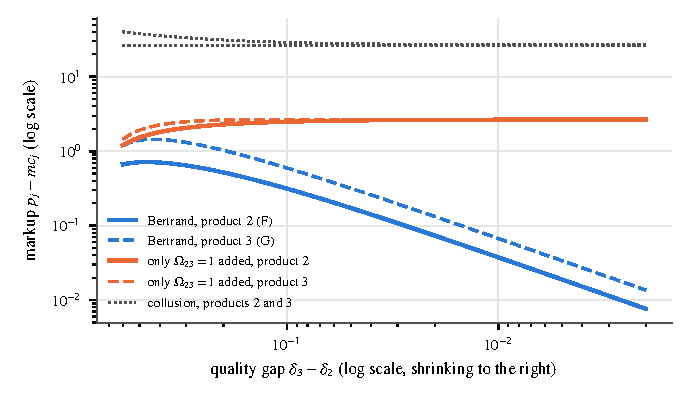
\includegraphics[width=0.74\textwidth]{figures/ch06/bresnahan_limit.pdf}
\caption{Markups of products 2 and 3 as their quality gap shrinks, in the seven-product design of
\cref{fig:06-bres-fig2}. Under Bertrand competition between their owners (blue) both markups fall in proportion to
the gap, as in \cref{prop:06-bertrand-limit}(a). If the Bertrand ownership matrix is changed only by letting
products 2 and 3 cooperate, $\Omega_{23} = 1$ (orange), the markups converge to a common positive value near 2.67,
as in part (b). Under full collusion (gray) they converge to about
26.7, the value given by \cref{eq:06-bres-mC}. Both axes are logarithmic. Computed with
\texttt{bresnahan\_fig2\_sim.py}.}
\label{fig:06-bres-limit}
\end{figure}

\subsubsection{The intuition and Bresnahan's Figure 2}\label{sec:06-bres-intuition}

Bresnahan states the intuition in two sentences \citep[p.~458]{Bresnahan1987}. If firms compete in prices, price is
near marginal cost for the products that have a close substitute sold by a competitor. If firms collude, the markup
on one firm's product hardly depends on whether its close substitutes are sold by competitors or by the firm itself.
\Cref{prop:06-bertrand-limit,prop:06-bres-collusion} make both sentences precise. Bresnahan adds a general point.
Conduct hypotheses differ in the comparative statics of price and quantity with respect to demand elasticities. So
conduct can be discerned even when marginal costs are unobserved, the same logic as the rotation argument of
\cref{ch:conduct}.

His Figure 2 illustrates the point with seven products in quality space and two firms, labelled G and F. We
recreate its design by solving the model. Products 2 and 3 are almost identical and belong to different firms.
Products 5, 6 and 7, at the top, all belong to G. \Cref{fig:06-bres-fig2} plots marginal cost and equilibrium prices
against quality under both conduct hypotheses, and \cref{fig:06-bres-fig2-orig} shows the original.\footnote{The
text of \citet[p.~466]{Bresnahan1987} describes the example differently from the figure. It says that ``Firm One
sells products 2, 4, and 5'' and that ``Firm Two sells product 3''. The prices of products 1 and 6 are held fixed,
because a third firm sells them. The figure labels the owners of products 1 to 7 as G, F, G, F, G, G, G. Our
recreation follows the figure. The economics is the same under both descriptions, because products 2 and 3 are
close neighbors owned by different firms.}

\begin{figure}[htbp]
\centering
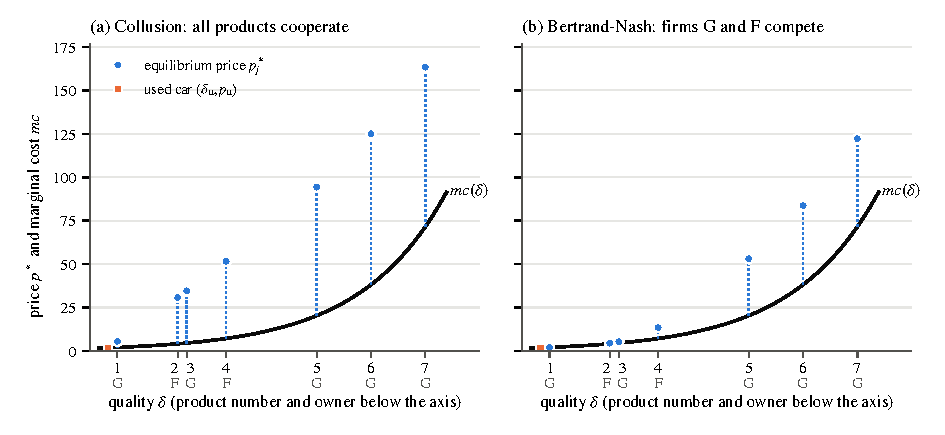
\includegraphics[width=\textwidth]{figures/ch06/bresnahan_fig2_sim.pdf}
\caption{Model-generated recreation of the design of \citet{Bresnahan1987}, Figure 2. Seven products with qualities
$\delta = (1, 2, 2.15, 2.8, 4.3, 5.2, 6.1)$ and owners G, F, G, F, G, G, G. Tastes are uniform with $\kappa = 1$ and
$\bar v = 48.3$. Marginal cost is $mc(\delta) = e^{0.7\delta}$, which is Bresnahan's $\psi e^{\delta}$ after a
rescaling of quality units. The used car has $\delta_{\mathrm u} = 0.85$ and $p_{\mathrm u} = mc(\delta_{\mathrm u})$.
Dots are equilibrium prices, and dotted segments are markups. Panel (a) solves \eqref{eq:06-bres-linear} with
$\Omega = \Omega^{\mathrm C}$ and panel (b) with the ownership matrix. Computed with \texttt{bresnahan\_fig2\_sim.py}.
The recreation copies the ownership labels of the original figure. Its markups need not match the original, which
Bresnahan drew as a sketch.}
\label{fig:06-bres-fig2}
\end{figure}

\begin{figure}[htbp]
\centering
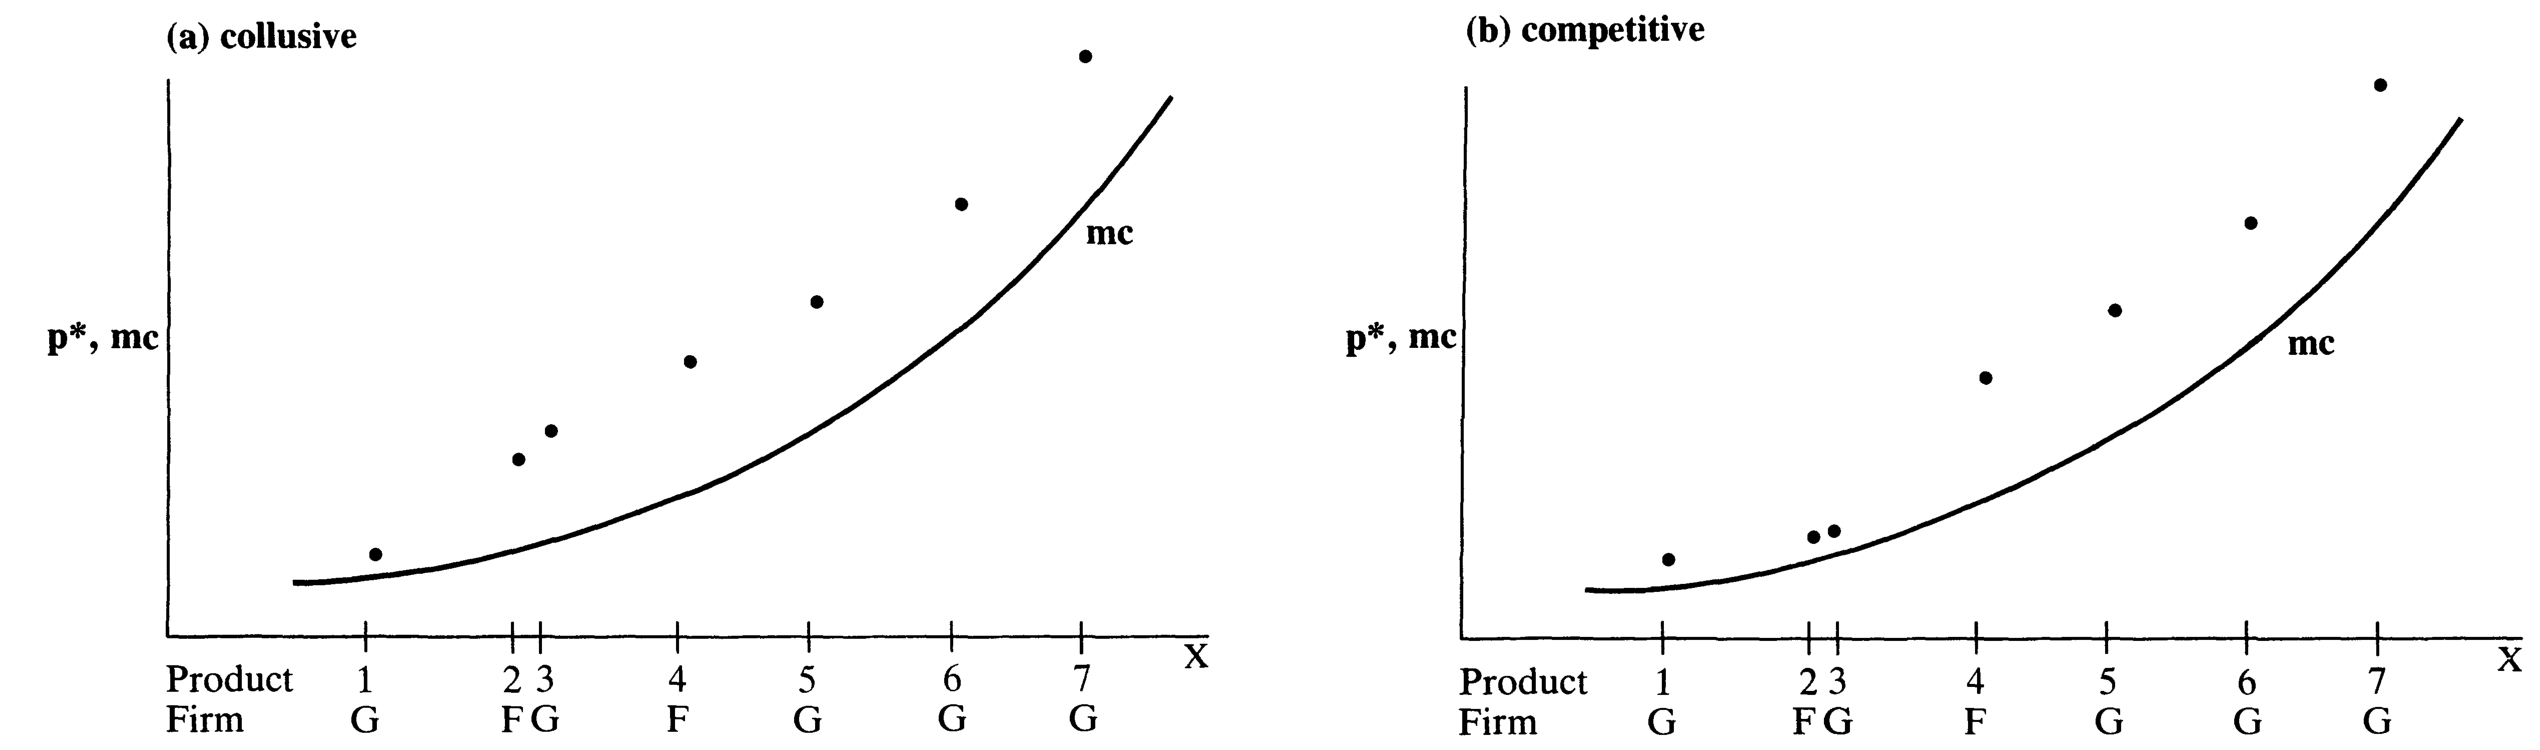
\includegraphics[width=\textwidth]{figures/ch06/bresnahan1987_fig2_orig.png}
\caption{Bresnahan's original illustration. Panel (a) shows collusive prices and panel (b) competitive prices, with
the marginal cost curve and the owner of each product below the quality axis. Source: \citet{Bresnahan1987},
Figure 2.}
\label{fig:06-bres-fig2-orig}
\end{figure}

The recreation shows three patterns. First, products 2 and 3 have markups of 26.65 and 30.05 under collusion and of
only 0.43 and 0.83 under Bertrand competition, so they sit on the cost curve in panel (b). Their rivalry is
fierce because they are close substitutes owned by different firms. Second, products 5, 6 and 7 keep between 44 and
55 percent of their collusive markups under Bertrand competition. They are distant from rivals and owned by one firm.
By \cref{rem:06-bres-topblock}, the price increments $p_6 - p_5$ and $p_7 - p_6$ and the quantities of products 6
and 7 are identical in the two panels. All three markups fall by the same amount, 41.28. Product 5 sells more under
Bertrand competition (7.61 against 5.50), because its lower cutoff falls when product 4 competes. Third, product 4,
owned by F and wedged between two G products at moderate distances, keeps 14 percent of its collusive markup. Most
of its Bertrand markup comes from the large markup of its upper neighbor, product 5, because prices are strategic
complements.

The recreation departs from Bresnahan's sketch in one visible respect. In his panel (b), products 4 to 7 keep nearly
all of their collusive markups. He writes that ``Products 4 and 5 change much less when the solution concept
changes'' \citep[p.~467]{Bresnahan1987}. In the solved model, product 4 keeps only 14 percent of its markup and
products 5 to 7 keep about half. Product 4 faces rival neighbors on both sides. Products 6 and 7 lose the same dollar
amount of markup as product 5, the lowest member of the top block (\cref{rem:06-bres-topblock}). Bresnahan's figure
is a sketch, and the robust contrast is the collapse of the markups of products 2 and 3.

The figure shows where the data can discriminate between the hypotheses. Regions of the quality ladder crowded with
products of different firms look very different under the two hypotheses. Regions with few firms change much less,
because market power is substantial even under competition. Bresnahan likens the large-car end of the mid-1950s
market, where GM produced most cars, to the region around products 4 and 5 of his example. He likens the
smaller-car segments to the region around products 1 and 2. There Ford, Chrysler, GM and, to a lesser extent, AMC
and the fringe were all present \citep[p.~467]{Bresnahan1987}. Bresnahan therefore expects the method to have statistical power in this industry. He also notes that the
method would be less revealing if every producer had a full product line \citep[p.~467]{Bresnahan1987}.
\Cref{rem:06-bres-power} makes this precise.

An earlier study supports this reading of the figure. \citet[pp.~1021--1022]{Bresnahan1989} summarizes
\citet{Bresnahan1981}, which fits the same vertical demand system to cross-sections of the 1977 and 1978 model
years. Its demand equation is the interior equation of \eqref{eq:06-bres-demand} (eq.~7 of the survey). Quality is
a hedonic function of length, weight, horsepower and other characteristics (eq.~8). The supply side is
\eqref{eq:06-bres-foc} under Bertrand conduct. Same-owner dummies on the two neighbors of each model play the role
of $\Omega_{j,j+1}$ and $\Omega_{j,j-1}$ (eq.~6$''$). The study reports two related findings. The large
price-cost margins appear on the larger vehicles, and the larger vehicles are much farther apart in quality space.
Products 5 to 7 of \cref{fig:06-bres-fig2} show the same pattern. They have no close rival, and they keep about
half of their collusive markups under Bertrand competition, while products 2 and 3 keep almost nothing. Bresnahan
adds that the finding confirms the view of industry observers based on accounting profits (footnote~13 of the
survey).

\subsection{Econometric specification and estimation}\label{sec:06-bres-estimation}

\casehead{Quality as an index of characteristics}
Quality is not observed. Bresnahan proxies it with a function of the physical characteristics (his eq.~22):
\begin{equation}\label{eq:06-bres-quality}
  \delta(x_j) = \sqrt{\beta_0 + x_j\beta},
\end{equation}
where $\beta_0$ and the vector $\beta$ are parameters. The interpretation comes from the hedonic model of
\citet{Rosen1974}, developed in \cref{sec:06-hedonic}. Consumers have preferences over characteristics, and firms
produce bundles of characteristics at costs that depend on them. The index is read as the expansion path of
efficient, cost-minimizing bundles. Each quality level is produced with the cheapest combination of characteristics
that delivers it. For this reason $\beta$ mixes information about tastes and technology, and its interpretation is
``clouded'' \citep[p.~467]{Bresnahan1987}. The square-root form is an arbitrary choice.

\casehead{Computing the model's predictions}
The parameters are $\theta = (\beta_0, \beta, \psi, \delta_{\mathrm u}, \bar v, \kappa)$, and the conduct hypothesis
fixes $\Omega$. For each trial value of $\theta$ the predictions are computed in three steps.
\begin{enumerate}
\item Compute every model's quality $\delta_j$ from \eqref{eq:06-bres-quality}.
\item Rank the models by quality, which determines who neighbors whom.
\item Solve the demand system \eqref{eq:06-bres-demand} and the first-order conditions \eqref{eq:06-bres-foc}
jointly for the predicted prices $p^*_j(\theta,\Omega)$ and quantities $q^*_j(\theta,\Omega)$, which amounts to the
linear system \eqref{eq:06-bres-linear}.
\end{enumerate}
The predictions depend only on parameters and on the exogenous characteristics. The used-car parameters are tied
together by \cref{ass:06-bres}(v), because the demand for the lowest-quality model \eqref{eq:06-bres-demand} is
overparameterized in $(\delta_{\mathrm u}, p_{\mathrm u})$. Bresnahan imposed $p_{\mathrm u} = mc(\delta_{\mathrm u})$
after initial experimentation showed the two were not easily distinguishable (p.~468).

\casehead{Errors and likelihood}
Observed prices and quantities equal the predictions plus additive, independent normal errors. Price errors have
variance $\sigma_p^2$. The error on aggregated quantity $m$ has variance $k_m\sigma_q^2$, from
\cref{sec:06-bres-data}, and price and quantity errors are independent. The likelihood is (his eq.~24)
\begin{equation}\label{eq:06-bres-lik}
  L(\theta,\sigma_p^2,\sigma_q^2)
  = \prod_{j=1}^{N_p}\frac{1}{\sqrt{2\pi\sigma_p^2}}\exp\Bigl[-\frac{(p_j - p_j^*)^2}{2\sigma_p^2}\Bigr]
    \prod_{m=1}^{N_q}\frac{1}{\sqrt{2\pi k_m\sigma_q^2}}
    \exp\Bigl[-\frac{\bigl(q_m - \sum_{j\in\mathcal I_m}q_j^*\bigr)^2}{2k_m\sigma_q^2}\Bigr],
\end{equation}
where $N_p$ and $N_q$ are the numbers of price and quantity observations and the predictions depend on
$(\theta,\Omega)$. The variances can be concentrated out. The log-likelihood is
\begin{equation*}
  \ln L = -\frac{N_p}{2}\ln(2\pi\sigma_p^2) - \frac{1}{2\sigma_p^2}\sum_{j}(p_j - p_j^*)^2
          - \frac{1}{2}\sum_m \ln(2\pi k_m\sigma_q^2) - \frac{1}{2\sigma_q^2}\sum_m \frac{(q_m - \sum_{j\in\mathcal I_m}q_j^*)^2}{k_m}.
\end{equation*}
Setting the derivative with respect to $\sigma_p^2$ to zero gives
$-\frac{N_p}{2\sigma_p^2} + \frac{1}{2\sigma_p^4}\sum_j (p_j - p_j^*)^2 = 0$, and similarly for $\sigma_q^2$. Hence
\begin{equation*}
  \hat\sigma_p^2(\theta) = \frac{1}{N_p}\sum_{j=1}^{N_p}(p_j - p_j^*)^2,
  \qquad
  \hat\sigma_q^2(\theta) = \frac{1}{N_q}\sum_{m=1}^{N_q}\frac{\bigl(q_m - \sum_{j\in\mathcal I_m}q_j^*\bigr)^2}{k_m}.
\end{equation*}
Substituting back gives the concentrated log-likelihood
\begin{equation}\label{eq:06-bres-conclik}
  \ell^c(\theta) = -\frac{N_p}{2}\ln\hat\sigma_p^2(\theta) - \frac{N_q}{2}\ln\hat\sigma_q^2(\theta)
  - \frac{1}{2}\sum_{m}\ln k_m - \frac{N_p + N_q}{2}\bigl(1 + \ln 2\pi\bigr).
\end{equation}
Maximum likelihood therefore chooses $\theta$ to minimize $N_p\ln\hat\sigma_p^2(\theta) + N_q\ln\hat\sigma_q^2(\theta)$.
Equivalently, it minimizes the product $(\hat\sigma_p^2)^{N_p}(\hat\sigma_q^2)^{N_q}$ of the mean squared price error
and the weighted mean squared quantity error. It is a form of nonlinear least squares for a system of two equations. All
estimation was done by numerical maximization.

\begin{remark}[A reduced-form error structure]\label{rem:06-bres-reducedform}
The errors in \eqref{eq:06-bres-lik} are appended to the equilibrium predictions. They are not structural demand or
cost shocks. Bresnahan calls this ``fully a reduced-form error structure'' (p.~469). It avoids the usual
endogeneity problem, because price never appears as a regressor and the predictions depend only on exogenous
characteristics. The cost of this choice is that the errors have no economic interpretation. A cost shock to one model would move
its neighbors' prices through the first-order conditions, which additive independent errors cannot capture.
\citet[p.~843]{BerryLevinsohnPakes1995} note that Bresnahan ``allows prices to be correlated with a linear
disturbance in an equilibrium pricing equation''. They add that he ``does not explicitly model the correlation
between prices and unobserved characteristics.'' Modelling an unobserved product characteristic $\xi_j$ and inverting market shares is
the response of \citet{Berry1994} and \citet{BerryLevinsohnPakes1995} (\cref{ch:logit,ch:blp}).
\end{remark}

\casehead{An irregular likelihood}
The likelihood is not continuous in the parameters. Predicted prices are continuous, but predicted quantities jump
at values of $\beta$ where two models, or a model and the used car, tie in quality. At such points the ranking
changes, and so does the set of neighbors. A discontinuous function cannot be concave, and the standard regularity
conditions for nonlinear regression fail. Bresnahan argues that ties are unlikely at the true parameter value, so
that limiting inference should go through (his footnote~9). He also reports that no local maxima caused trouble and
that the points of discontinuity were typically local minima, since they imply extreme predicted quantities
(footnote~10). Asymptotic normality of the estimators and of the test statistics remains unproven, as Appendix~B
acknowledges.

\casehead{Two further specifications}
Two more models serve as alternatives in the tests. The first is the log-linear hedonic model of
\citet{CowlingCubbin1971}, estimated on the British car market. Predicted prices and quantities follow a recursive
structure (his eqs.~25--26):
\begin{equation}\label{eq:06-bres-hedonic}
  p_j^* = \exp\bigl(a_0 + x_j a\bigr),
  \qquad
  q_j^* = \exp\bigl(l_0 + l_1(p_j - p_j^*)\bigr),
\end{equation}
where we write $a_0$, $a$, $l_0$ and $l_1$ for Bresnahan's $\alpha_0$, $\alpha_j$, $\lambda_0$ and $\lambda_1$. The
price equation adds GM and Ford dummies, following authors who use firm dummies as a proxy for market power. The
model has the same error and aggregation structure as the oligopoly models. \citet{Rosen1974} interprets a hedonic
price function as the equilibrium of a perfectly competitive, continuously differentiated market. The hedonic model,
``or something like it'', should hold if list prices were set in some nonmaximizing way (p.~470). It differs
radically from the oligopoly models. The second alternative, called ``Products'', is the opposite. It follows the
oligopoly model exactly but treats every model as if a separate firm made it, so $\Omega = I$. Neither is an
appealing story of the industry. Both are useful as tests, because an oligopoly model that survives against them
is more credible.

\subsection{Testing non-nested conduct hypotheses}\label{sec:06-bres-cox}

Collusion and Bertrand competition are non-nested hypotheses. They impose different matrices $\Omega$, and no
restriction on the parameters turns one model into the other. The hedonic model is a different family altogether.
A classical likelihood ratio test, which compares a model with a restricted version of itself, does not apply.
Bresnahan uses the non-nested test of \citet{Cox1961} in the regression form of \citet{PesaranDeaton1978}
\citep[p.~470]{Bresnahan1987}.

\casehead{The Cox statistic}
Let $H_0$ and $H_1$ be two parametric models for the same data, with maximized log-likelihoods $L_0$ and $L_1$. The
\emph{Cox statistic} for testing $H_0$ against $H_1$ is the observed log-likelihood ratio minus an estimate of its
expectation under $H_0$,
\begin{equation}\label{eq:06-bres-coxstat}
  T_0 = (L_0 - L_1) - \hat\E_0\bigl[L_0 - L_1\bigr].
\end{equation}
The expectation is evaluated at the estimate of $\theta_0$. It replaces the parameters of $H_1$ by their
\emph{pseudo-true values}, the probability limit of the $H_1$ estimator when the data come from $H_0$. Under $H_0$ the
standardized statistic is asymptotically standard normal. A significantly negative $T_0$ means that $H_1$ fits better
than it should if $H_0$ were true, which is evidence against $H_0$ in the direction of $H_1$. A significantly positive
$T_0$ means that $H_1$ fits worse than $H_0$ predicts. The test is two-tailed, so this also rejects $H_0$, whose
likelihood is ``too large'' relative to $H_1$. The test is not symmetric. Testing $H_1$ against $H_0$ is a different
test, so both models can be rejected, or neither. The next proposition gives the statistic for regression models.

\begin{proposition}[Cox statistic for non-nested regressions]\label{prop:06-bres-cox}
Let $y \in \R^N$, $H_0: y = f_0(\theta_0) + u$ and $H_1: y = f_1(\theta_1) + w$, with $u \sim N(0,\sigma_0^2 I_N)$ under
$H_0$, smooth mean functions, and parameter vectors of fixed dimension. Let $s_0^2$ and $s_1^2$ be the maximum
likelihood residual variances under the two models. Fit $H_1$ to the fitted values of $H_0$: let
$\hat\theta_{10}$ minimize $\|f_0(\hat\theta_0) - f_1(\theta_1)\|^2$, let $\hat d = f_0(\hat\theta_0) - f_1(\hat\theta_{10})$,
and define
\begin{equation*}
  \phi^2 = \frac{1}{N}\|\hat d\|^2,
  \qquad s_{10}^2 = s_0^2 + \phi^2,
  \qquad \tilde\phi = \frac{1}{N}\hat d^\top M_0\hat d,
\end{equation*}
where $M_0 = I_N - F_0(F_0^\top F_0)^{-1}F_0^\top$ and $F_0 = \frac{\partial f_0(\hat\theta_0)}{\partial\theta_0^\top}$. Then
\begin{equation*}
  T_0 = \frac{N}{2}\ln\frac{s_1^2}{s_{10}^2}.
\end{equation*}
If $H_0$ is true, $H_1$ does not contain the true mean function, and standard regularity conditions hold, then
\begin{equation*}
  \frac{T_0}{\sqrt{V_0}} \xrightarrow{d} N(0,1),
  \qquad
  V_0 = \frac{N\tilde\phi\, s_0^2}{s_{10}^4}.
\end{equation*}
\end{proposition}

\begin{proof}[Proof sketch]
The concentrated log-likelihood of a normal regression is $-\frac{N}{2}\ln s^2$ plus a constant common to both
models. Hence
\begin{equation*}
  L_0 - L_1 = \frac{N}{2}\ln\frac{s_1^2}{s_0^2}.
\end{equation*}
Under $H_0$, $s_1^2$ converges to $\sigma_0^2 + \phi_*^2$, where $\phi_*^2$ is the limit of $\phi^2$, the part of the
$H_0$ mean that $H_1$ cannot fit. The estimated expectation of $L_0 - L_1$ is therefore
$\frac{N}{2}\ln\frac{s_{10}^2}{s_0^2}$, and subtracting it gives $T_0$.

For the distribution we expand to first order around the true $\theta_0$ and the pseudo-true value
$\theta_{10}^*$. Write $f_0 = f_0(\theta_0)$ and $d = f_0 - f_1(\theta_{10}^*)$. Let $F_1$ be the gradient of $f_1$ at
$\theta_{10}^*$, define $M_1$ from $F_1$ as $M_0$ is defined from $F_0$, and let $P_k = I_N - M_k$ be the projection
onto the columns of $F_k$. The first-order condition
defining $\theta_{10}^*$ is $F_1^\top d = 0$, so $M_1d = d$. Four steps follow.
\begin{enumerate}
\item Fitting $H_1$ to $y = f_0 + u$ leaves residuals $M_1(d + u)$ to first order. Hence
$Ns_1^2 \approx \|d\|^2 + 2d^\top u + u^\top M_1 u$.
\item Fitting $H_0$ leaves residuals $M_0u$, so $Ns_0^2 \approx u^\top M_0 u$.
\item The fitted values of $H_0$ are $f_0 + P_0u$ to first order. Fitting $H_1$ to them, as in step 1, gives
$N\phi^2 \approx \|d\|^2 + 2d^\top P_0u + u^\top P_0M_1P_0u$.
\item Subtracting, $N(s_1^2 - s_{10}^2) \approx 2d^\top M_0 u + R$, where $R$ collects quadratic forms in $u$ on spaces of
fixed dimension and is bounded in probability. The term $d^\top M_0u$ is of order $\sqrt N$ because
$\|d\|^2$ grows like $N$.
\end{enumerate}
Since $\ln\frac{s_1^2}{s_{10}^2} \approx \frac{s_1^2 - s_{10}^2}{s_{10}^2}$, the statistic satisfies
\begin{equation*}
  T_0 \approx \frac{d^\top M_0u}{\sigma_0^2 + \phi_*^2},
  \qquad
  \Var_0\bigl(d^\top M_0 u\bigr) = \sigma_0^2\, d^\top M_0 d .
\end{equation*}
The leading term is normal with mean zero and variance $\frac{\sigma_0^2\, d^\top M_0 d}{(\sigma_0^2 + \phi_*^2)^2}$. Its
plug-in estimate is $V_0$, since $N\tilde\phi$ estimates $d^\top M_0d$. \citet{Pesaran1974} and
\citet{PesaranDeaton1978} give the regularity conditions and the multivariate version.
\end{proof}

The proof explains the two auxiliary regressions in Bresnahan's Appendix B. The first fits $H_1$ to the fitted
values of $H_0$, which he calls the ``phony-data regression''. Its residual variance $\phi^2$ measures how far $H_1$
is from $H_0$. The second regresses the phony-data residuals on the derivatives of $H_0$'s predictions. Its
residual variance $\tilde\phi$ removes the part of the distance that a small change in $\theta_0$ could absorb.
The intuition of the test is simple: $H_0$ is rejected if $H_1$ explains a significant part of $H_0$'s
residuals \citep[p.~471]{Bresnahan1987}.

\casehead{Bresnahan's formulas}
Bresnahan's models have two equations with independent errors, and the quantity equation is weighted by
$\frac{1}{k_m}$. The concentrated log-likelihood \eqref{eq:06-bres-conclik} has the same weights under every model,
so the terms in $k_m$ cancel from all likelihood ratios. The contributions of the two equations add. Let $s^2_{jp}$
and $s^2_{jq}$ be the estimated price and quantity error variances under $H_j$, for $j = 0, 1$ (his eqs.~B.1--B.2).
The phony-data regression fits $H_1$ to the predictions of $H_0$ and yields variances $\phi^2_p$ and $\phi^2_q$. Then
(his eqs.~B.3--B.5)\footnote{Equation (B.4) is printed as $s^2_{10q} \equiv s^2_{0p} + \phi^2_q$. The subscript $0p$ is
a misprint for $0q$, by analogy with (B.3) and with \cref{prop:06-bres-cox}.}
\begin{equation}\label{eq:06-bres-T0}
  s^2_{10p} = s^2_{0p} + \phi^2_p,
  \qquad
  s^2_{10q} = s^2_{0q} + \phi^2_q,
  \qquad
  T_0 = \frac{N_p}{2}\ln\frac{s^2_{1p}}{s^2_{10p}} + \frac{N_q}{2}\ln\frac{s^2_{1q}}{s^2_{10q}} .
\end{equation}
The second regression takes the residuals of the phony-data regression and regresses them linearly on the
derivatives of the $H_0$ predictions with respect to the $H_0$ parameters. Its residual variances are
$\tilde\phi_p$ and $\tilde\phi_q$, which Bresnahan writes as $\phi p$ and $\phi q$. They are variances in their own
right. They are not the square roots of $\phi^2_p$ and $\phi^2_q$. The asymptotic variance of $T_0$ is (his eq.~B.6)
\begin{equation}\label{eq:06-bres-V0}
  V_0(T_0) = N_p\tilde\phi_p\,\frac{s^2_{0p}}{s^4_{10p}} + N_q\tilde\phi_q\,\frac{s^2_{0q}}{s^4_{10q}},
\end{equation}
and the test statistic is $\frac{T_0}{\sqrt{V_0(T_0)}}$.\footnote{Appendix B prints the statistic as the ratio of $T_0$ to $V(T_0)$, without a square root. The text
(p.~470) divides the deviation of the likelihood ratio from its mean ``by its standard deviation''.
\Cref{prop:06-bres-cox} confirms that the square root is required for an asymptotically standard normal statistic. We
read the printed ratio as shorthand.} Each term of \eqref{eq:06-bres-T0} and \eqref{eq:06-bres-V0} is the
single-equation formula of \cref{prop:06-bres-cox}. Bresnahan's footnote~11 notes that the Pesaran-Deaton formulas were
altered slightly to account for the aggregation of quantities.

\begin{table}[htbp]
\centering
\caption{Cox test statistics for each maintained hypothesis against each alternative, 1954--1956}
\label{tab:06-bres-cox}
\small
\begin{tabular}{@{}lrrrr@{}}
\toprule
 & \multicolumn{4}{c}{Alternative hypothesis $H_1$} \\
\cmidrule(l){2-5}
Maintained hypothesis $H_0$ & Collusion & Nash-Competition & ``Products'' & Hedonic \\
\midrule
\multicolumn{5}{@{}l}{\textit{(a) 1954}} \\
Collusion        & $\cdot$     & 0.8951      & 0.9464      & $-1.934$ \\
Nash-Competition & $-2.325^{*}$ & $\cdot$    & $-0.8878$   & $-2.819^{*}$ \\
``Products''     & $-3.978^{*}$ & $3.029^{*}$ & $\cdot$    & $-1.604$ \\
Hedonic          & $-12.37^{*}$ & $-10.94^{*}$ & $-13.02^{*}$ & $\cdot$ \\
\addlinespace
\multicolumn{5}{@{}l}{\textit{(b) 1955}} \\
Collusion        & $\cdot$     & $-10.36^{*}$ & $-9.884^{*}$ & $-13.36^{*}$ \\
Nash-Competition & $-1.594$    & $\cdot$      & 1.260        & 0.6341 \\
``Products''     & $-0.7598$   & $-4.379^{*}$ & $\cdot$      & $-1.527$ \\
Hedonic          & $-3.353^{*}$ & $-8.221^{*}$ & $-5.950^{*}$ & $\cdot$ \\
\addlinespace
\multicolumn{5}{@{}l}{\textit{(c) 1956}} \\
Collusion        & $\cdot$     & 1.227        & 0.8263       & 1.629 \\
Nash-Competition & $-2.426^{*}$ & $\cdot$     & $-4.586^{*}$ & 0.8314 \\
``Products''     & $-3.153^{*}$ & 0.9951      & $\cdot$      & $4.731^{*}$ \\
Hedonic          & $-5.437^{*}$ & $-9.671^{*}$ & $-11.58^{*}$ & $\cdot$ \\
\bottomrule
\end{tabular}

\smallskip
\begin{minipage}{0.92\textwidth}
\footnotesize
\emph{Notes:} Reproduced from \citet[Table III, p.~471]{Bresnahan1987}. Each entry is the standardized Cox
statistic $\frac{T_0}{\sqrt{V_0}}$ for testing the row model against the column model, asymptotically standard
normal under the row model. A dot marks the diagonal. Asterisks are ours and mark rejection at the 5 percent level
in a two-tailed test, $\bigl|\frac{T_0}{\sqrt{V_0}}\bigr| > 1.96$. Negative values indicate that the alternative fits better than the maintained
model predicts. ``Products'' treats every model as a separate firm ($\Omega = I$). The hedonic model is
\eqref{eq:06-bres-hedonic}.
\end{minipage}
\end{table}

\casehead{Results}
\Cref{tab:06-bres-cox} reproduces the test results. In 1954 the hedonic model is rejected against every other
model. ``Products'' is rejected against both oligopoly models but not against the hedonic model.
Nash-Competition is rejected against Collusion ($-2.325$) and against the hedonic model ($-2.819$). Collusion is the
only model that escapes rejection against every alternative. Its statistic against the hedonic model, $-1.934$, is
close to the 5 percent cutoff of 1.96 but below it in absolute value. The 1956 results resemble those of 1954. Collusion is not
rejected against any alternative, and every other model is rejected at least once. Nash-Competition, for example,
is rejected against Collusion ($-2.426$) and against ``Products'' ($-4.586$).

The 1955 results are reversed. Collusion is rejected against all three alternatives, with statistics of $-10.36$,
$-9.884$ and $-13.36$. Nash-Competition is rejected against none. The other models are rejected as in the
surrounding years. ``Products'' is rejected against Nash-Competition, and the hedonic model against everything.
Some rejections have positive signs, as for ``Products'' against Nash-Competition in 1954 ($3.029$) and against the
hedonic model in 1956 ($4.731$). These reject because the likelihood of ``Products'' is too large relative to the
alternative, a possibility Bresnahan's footnote~12 points out for the two-tailed test.

Bresnahan stresses that the test results and the output expansion are independent evidence. Each year is estimated
separately, and no cross-year restriction, for example on the location of the demand curve, forces the competitive
model to be chosen in the high-quantity year. The coincidence of the reversal with the boom is therefore
informative \citep[p.~472]{Bresnahan1987}. The results are also robust to the two added specifications, which are
rejected throughout. The hedonic model is the cleanest of these rejections, since its likelihood is regular and the
caveat on asymptotic normality does not apply to it.

\subsection{Estimates}\label{sec:06-bres-estimates}

\begin{table}[t]
\centering
\caption{Parameter estimates under the maintained conduct hypotheses, 1954--1956}
\label{tab:06-bres-iv}
\small
\begin{tabular}{@{}lccc@{}}
\toprule
Parameter & 1954 (Collusion) & 1955 (Bertrand) & 1956 (Collusion) \\
\midrule
\multicolumn{4}{@{}l}{\textit{Quality index $\delta(x) = \sqrt{\beta_0 + x\beta}$}} \\
Constant $\beta_0$          & 47.91    & 48.28    & 50.87 \\
                            & (32.8)   & (43.2)   & (29.4) \\
Weight (thousands of lb)    & 0.3805   & 0.5946   & 0.5694 \\
                            & (0.332)  & (0.145)  & (0.374) \\
Length (thousands of in.)   & 0.1819   & 0.1461   & 0.1507 \\
                            & (0.128)  & (0.059)  & (0.146) \\
Horsepower (hundreds)       & 2.665    & 3.350    & 3.248 \\
                            & (0.692)  & (0.535)  & (0.620) \\
Cylinders                   & $-0.7387$ & $-0.9375$ & $-0.9639$ \\
                            & (0.205)  & (0.115)  & (0.186) \\
Hardtop dummy               & 0.9445   & 0.4531   & 0.4311 \\
                            & (0.379)  & (0.312)  & (0.401) \\
\addlinespace
\multicolumn{4}{@{}l}{\textit{Demand and supply}} \\
Marginal cost scale $\psi$  & 0.1753   & 0.1747   & 0.1880 \\
                            & (0.024)  & (0.020)  & (0.035) \\
Used-car quality $\delta_{\mathrm u}$ & 4.593 & 3.911 & 4.441 \\
                            & (1.49)   & (2.08)   & (1.46) \\
Upper endpoint $\bar v$     & $1.92\times10^{7}$ & $2.41\times10^{7}$ & $2.83\times10^{7}$ \\
                            & $(8.44\times10^{6})$ & $(9.21\times10^{6})$ & $(7.98\times10^{6})$ \\
Taste density $\kappa$      & 0.4108   & 0.4024   & 0.4075 \\
                            & (0.138)  & (0.184)  & (0.159) \\
\bottomrule
\end{tabular}

\smallskip
\begin{minipage}{0.86\textwidth}
\footnotesize
\emph{Notes:} Reproduced from \citet[Table IV, p.~472]{Bresnahan1987}. Asymptotic standard errors in parentheses.
Each column uses the conduct hypothesis not rejected in \cref{tab:06-bres-cox}. The mapping to Bresnahan's symbols
is: $\psi$ is his $\mu$, $\delta_{\mathrm u}$ is his $\gamma$, $\bar v$ is his $V_{\max}$, and $\kappa$ is his
$\delta$. The paper does not report the numbers of price and quantity observations.
\end{minipage}
\end{table}

\Cref{tab:06-bres-iv} reports the estimates under the specification that survives the tests in each year: Collusion
for 1954 and 1956 and Bertrand for 1955. The three columns are close. The marginal-cost scale is
0.1753, 0.1747 and 0.1880. The taste density is 0.4108, 0.4024 and 0.4075. The quality-index coefficients are close
in size and sign across years. The estimated primitives barely move, so the change in conduct alone captures the distinct
features of 1955.

\begin{table}[t]
\centering
\caption{Parameter estimates when one conduct hypothesis is imposed in every year}
\label{tab:06-bres-v}
\footnotesize
\setlength{\tabcolsep}{4pt}
\begin{tabular}{@{}lcccccc@{}}
\toprule
 & \multicolumn{3}{c}{(i) Collusive specification} & \multicolumn{3}{c}{(ii) Bertrand specification} \\
\cmidrule(lr){2-4}\cmidrule(l){5-7}
Parameter & 1954 & 1955 & 1956 & 1954 & 1955 & 1956 \\
\midrule
Constant $\beta_0$ & 47.91 & $-23.37$ & 50.87 & 31.64 & 48.28 & 33.23 \\
  & (32.8) & (24.5) & (29.4) & (29.9) & (43.2) & (17.8) \\
Weight & 0.3805 & 0.0103 & 0.5694 & 0.9311 & 0.5946 & $6.23\times10^{-3}$ \\
  & (0.332) & $(5.43\times10^{-2})$ & (0.374) & (0.210) & (0.145) & $(8.73\times10^{-4})$ \\
Length & 0.1819 & $-2.88\times10^{-3}$ & 0.1507 & 0.1474 & 0.1461 & 0.1605 \\
  & (0.128) & (0.102) & (0.146) & (0.038) & (0.059) & (0.149) \\
Horsepower & 2.665 & 0.1165 & 3.248 & 4.962 & 3.350 & $2.972\times10^{-2}$ \\
  & (0.692) & (0.106) & (0.620) & (0.676) & (0.535) & $(1.47\times10^{-2})$ \\
Cylinders & $-0.7387$ & $-1.309$ & $-0.9639$ & $-0.8846$ & $-0.9375$ & $-0.9078$ \\
  & (0.205) & (1.52) & (0.186) & (0.194) & (0.115) & (0.256) \\
Hardtop & 0.9445 & 1.468 & 0.4311 & $-0.2474$ & 0.4531 & 0.5282 \\
  & (0.379) & (1.08) & (0.401) & (0.464) & (0.312) & (0.249) \\
$\psi$ & 0.1753 & 1.344 & 0.1880 & 0.2518 & 0.1747 & 0.2902 \\
  & (0.024) & (0.151) & (0.035) & (0.074) & $(0.312)^{a}$ & $(0.249)^{a}$ \\
$\delta_{\mathrm u}$ & 4.593 & 1.604 & 4.441 & 6.352 & 3.911 & 1.204 \\
  & (1.49) & (4.83) & (1.46) & (3.54) & (2.08) & (3.19) \\
$\bar v$ & $1.92\times10^{7}$ & $1.46\times10^{8}$ & $2.83\times10^{7}$ & $9.81\times10^{5}$ & $2.41\times10^{7}$ & $1.03\times10^{6}$ \\
  & $(8.44\times10^{6})$ & $(6.74\times10^{6})$ & $(7.98\times10^{6})$ & $(8.78\times10^{6})$ & $(9.21\times10^{6})$ & $(8.90\times10^{6})$ \\
$\kappa$ & 0.4108 & $5.75\times10^{-2}$ & 0.4075 & 5.04 & 0.4024 & 7.334 \\
  & (0.138) & $(8.28\times10^{-2})$ & (0.159) & (1.21) & (0.184) & (2.46) \\
\bottomrule
\end{tabular}

\smallskip
\begin{minipage}{0.95\textwidth}
\footnotesize
\emph{Notes:} Reproduced from \citet[Tables V(i) and V(ii), pp.~473--474]{Bresnahan1987}. Asymptotic standard errors in
parentheses. Symbols as in \cref{tab:06-bres-iv}. $^{a}$~Printed as in the source. These two standard errors
duplicate the hardtop standard errors directly above them, (0.312) and (0.249). Table IV reports (0.020) for the
same 1955 estimate of $\psi$, so the printed values are probably typesetting errors. The paper also reports Table
V(iii) for the hedonic model and Table V(iv) for ``Products''.
\end{minipage}
\end{table}

\Cref{tab:06-bres-v} tells the opposite story. When one conduct hypothesis is imposed in all three years, the
parameters must explain 1955 by themselves, and they behave erratically. Under the collusive specification the 1955
column departs from its neighbors. The marginal-cost scale $\psi$ is an order of magnitude larger, 1.344 against
0.1753 and 0.1880. The taste density $\kappa$ is an order of magnitude smaller, 0.0575 against about 0.41. The upper
endpoint $\bar v$ jumps to $1.46\times10^{8}$, and length receives a negative coefficient. The parameters must absorb
the low prices and high output that collusive pricing cannot generate with stable primitives.

The Bertrand specification is ``similarly chaotic'' \citep[p.~473]{Bresnahan1987}. Now 1954 and 1956 are the odd
years. The 1954 column has the only negative hardtop coefficient estimated in any year under any specification. In 1956 the
weight and horsepower coefficients collapse toward zero, to $6.23\times10^{-3}$ and $2.972\times10^{-2}$. Relative to
the surrounding years, tastes in 1955 are spread ``at one tenth the density over ten times the range'' (p.~475).
The comparison is with the Bertrand estimates for 1954 and 1956, where $\kappa$ is 5.04 and 7.334 and $\bar v$ is near
$10^{6}$. The 1955 values, 0.4024 and $2.41\times10^{7}$, are those of \cref{tab:06-bres-iv}, since both tables estimate 1955
under Bertrand.
Bresnahan sums up the comparison in one sentence: ``It is change of behavioral assumption, not change of parameter
values, that provides a reasonable empirical explanation of 1955'' (p.~475).

The lesson is general. A misspecified conduct assumption does not disappear. It is absorbed into the estimated
primitives, which then become unstable across periods and implausible in level. Stability of demand and cost
parameters across periods is therefore informative about conduct. \Cref{tab:06-bres-iv} is built from the two panels
of \cref{tab:06-bres-v}, and only the combination left unrejected by the tests produces a consistent picture.

The magnitudes in \cref{tab:06-bres-iv} have sensible readings \citep[p.~475]{Bresnahan1987}. The quality-index
coefficients have the signs and sizes one expects from hedonic regressions. The negative cylinders coefficient is
familiar from that literature too. Econometrically, horsepower and cylinders are highly collinear. Economically,
the cylinders variable captures the fall in the cost of horsepower after the introduction of the V-8 engine.

The demand parameters describe very diverse tastes for quality. The eight million buyers of 1955 had tastes $v$
between $4.24\times10^{6}$ and $2.4\times10^{7}$. In Bresnahan's words, the distribution was ``20 million wide and 0.4
deep'', and 20 million times 0.4 gives the eight million buyers. Bresnahan cautions that this may be an artifact of
the constant density. The same numbers imply a potential market of $\kappa\bar v = 0.4024\times 2.41\times10^{7}
\approx 9.7$ million in 1955, of whom about 1.7 million (those with $v$ below $4.24\times10^{6}$) chose the used
car. The used-car quality $\delta_{\mathrm u}$ is around 4 in each year, while the lowest new-car quality is around
9. New and used cars are thus not close substitutes. The parameter $\psi$ only converts quality units into money in
the marginal-cost function.

Two further readings concern 1956. The 1955 purchases do not seem to have depressed 1956 demand. Both $\kappa$ and $\bar v$
are slightly larger in 1956 than in 1955, and the 1954 and 1956 demand parameters are very similar. The used-car
quality rises from 3.911 in 1955 to 4.441 in 1956 (it was 4.593 in 1954), which Bresnahan reads as considerable competition from the used-car
market in 1956. For comparison, the hedonic model's quantity equation gives price coefficients $l_1$ of $-3.742$
(0.640), $-1.312$ (0.787) and $-3.322$ (0.715) in 1954, 1955 and 1956 (Table V(iii)). The 1955 coefficient is the
smallest in absolute value and the least precise.

\subsection{Counterfactual, fit and residuals}\label{sec:06-bres-fit}

\casehead{Collusion in 1955 as a counterfactual}
The estimates allow a simple decomposition of the 1955 expansion into demand and conduct. Bresnahan computes the
equilibrium with the 1955 parameters, which were estimated under Bertrand, but with the collusive solution. The
counterfactual prices are about one-half of one percent above the average of 1954 and 1956. Predicted 1955 unit
sales are 7.1 million, 25.5 percent above the 1954 and 1956 average, instead of the actual 40.4 percent. The change
in conduct thus accounts for about 0.8 million cars, the difference between 7.9 and 7.1 million. Bresnahan compares
this with the largest residual in the demand system of \citet{Chow1960}, $+0.6$ million units, which falls in 1955.
The two magnitudes are comparable. A supply-side change of the size implied by the price war is thus of the same
order as the part of 1955 that demand models could not explain.

\begin{table}[htbp]
\centering
\caption{Fit of the four models and residuals of the Big Three, 1954--1956}
\label{tab:06-bres-fit}
\small
\begin{tabular}{@{}lcccccc@{}}
\toprule
\multicolumn{7}{@{}l}{\textit{(a) $R^2$ of the price ($p$) and quantity ($q$) equations (Table VI)}} \\
\addlinespace
 & \multicolumn{2}{c}{1954} & \multicolumn{2}{c}{1955} & \multicolumn{2}{c}{1956} \\
\cmidrule(lr){2-3}\cmidrule(lr){4-5}\cmidrule(l){6-7}
Model & $p$ & $q$ & $p$ & $q$ & $p$ & $q$ \\
\midrule
Collusion    & 0.94 & 0.62 & 0.92 & 0.58 & 0.96 & 0.61 \\
Bertrand     & 0.91 & 0.62 & 0.96 & 0.64 & 0.93 & 0.62 \\
``Products'' & 0.90 & 0.62 & 0.88 & 0.59 & 0.92 & 0.61 \\
Hedonic      & 0.89 & 0.71 & 0.88 & 0.73 & 0.88 & 0.71 \\
\midrule
\multicolumn{7}{@{}l}{\textit{(b) Average residual of each firm minus the average of all other firms (Table VII)}} \\
\addlinespace
 & \multicolumn{2}{c}{1954 (Collusion)} & \multicolumn{2}{c}{1955 (Bertrand)} & \multicolumn{2}{c}{1956 (Collusion)} \\
\cmidrule(lr){2-3}\cmidrule(lr){4-5}\cmidrule(l){6-7}
Firm & Price & Quantity & Price & Quantity & Price & Quantity \\
\midrule
GM       & 20.92    & $-99.6$ & 28.80   & $-82.86$ & 21.48    & $-68.73$ \\
Ford     & $-12.33$ & 60.2    & $-6.28$ & 22.97    & $-11.02$ & 19.06 \\
Chrysler & $-13.16$ & 96.89   & $-9.33$ & 64.47    & $-17.19$ & 11.94 \\
\bottomrule
\end{tabular}

\smallskip
\begin{minipage}{0.92\textwidth}
\footnotesize
\emph{Notes:} Panel (a) reproduces \citet[Table VI, p.~476]{Bresnahan1987}. Because of the heteroskedasticity, the quantity
$R^2$ is defined as a fraction of explained variance, $R^2_q = \frac{s^2_q - \hat\sigma^2_q}{s^2_q}$. Here $s^2_q$ is the
second raw moment of the quantity data, computed under the same heteroskedastic variance structure as the models. Panel (b) reproduces Table VII (p.~477), computed from the unrejected specification in each
year. Price residuals are in dollars and quantity residuals in cars. ``All other firms'' includes the other two
firms of the Big Three.
\end{minipage}
\end{table}

\casehead{Fit}
Panel (a) of \cref{tab:06-bres-fit} gives part of the intuition behind the tests. The reversal between Collusion and
Bertrand appears as a reversal in $R^2$. In the price equation the unrejected model fits better in every year: 0.94
against 0.91 in 1954, 0.96 against 0.92 in 1955, and 0.96 against 0.93 in 1956. In the quantity equation it fits
better in 1955 (0.64 against 0.58) and equally well in 1954 (0.62 each).\footnote{Bresnahan writes that ``in each
year, the model not rejected explains more variance in both equations'' (p.~477). In 1956, however, Table VI gives
a quantity $R^2$ of 0.61 for Collusion and 0.62 for Bertrand, so the statement holds strictly only for the price
equation.} The hedonic model fits quantities better in every year, with $R^2_q$ of 0.71 to 0.73, yet the oligopoly
model left unrejected in each year is not rejected against it. Bresnahan concludes that the price equation provides most of the power of the
tests. His footnote~14 gives two reasons to read these $R^2$ values with care. The oligopoly models have no constant
in the quantity equation, by \eqref{eq:06-bres-demand}. In the price equation, marginal cost explains much of the
cross-sectional variance, so the price $R^2$ would be high even if little of the markup were explained.

\casehead{Residuals by firm}
Panel (b) compares the average residuals of each of the Big Three with those of all other firms. Since ``all other
firms'' for Ford and Chrysler includes GM, the clearest message concerns GM. Its average price residual is 20.92,
28.80 and 21.48 dollars, and its average quantity residual is $-99.6$, $-82.86$ and $-68.73$ cars. Bresnahan
summarizes these as overpredicting GM prices by about \$30, out of the \$1,500 price of a typical car. He also
describes them as underpredicting GM sales by about 100 units, out of typical sales near 60,000.\footnote{The paper does not define the
sign of a residual. Bresnahan's wording matches residuals defined as predicted minus observed values. Under the more
common convention, observed minus predicted, the same numbers would mean that the models underpredict GM prices and
overpredict GM sales. The magnitudes are unaffected. Note also that the printed price residuals, \$21 to \$29, are
somewhat below the \$30 of the text.} The errors are small, but they suggest that GM had a cost or quality advantage.
Bresnahan therefore estimated two broader specifications for each oligopoly model. One adds a GM dummy to the quality
index. The other gives GM its own marginal-cost scale. Neither GM parameter is significant in any unrejected
specification, and no Cox test result is reversed. Either parameter does make the GM residuals much closer to zero.

\subsection{Robustness}\label{sec:06-bres-robust}

Besides the GM extensions, Bresnahan reports two generalizations aimed at the most obvious weaknesses of the model.

\casehead{Quality measured with error}
The tests depend on which products are neighbors. Small errors in the imputed qualities could change the ranking of
products, and with it the pattern of same-firm and rival neighbors. Robert Masson raised this concern (footnote~15).
Following \citet{Bresnahan1981}, the quality index is rewritten as observed with error,
\begin{equation}\label{eq:06-bres-qerror}
  \delta(x_j) = \sqrt{\beta_0 + x_j\beta} + \zeta_j,
\end{equation}
where we write $\zeta_j$ for Bresnahan's $\varepsilon_x$.\footnote{The printed formula on p.~478 reads
$\sqrt{\beta_0 + \varepsilon_j\beta_jZ_j} + \varepsilon_x$. The first $\varepsilon_j$ is a misprint for the summation sign.}
Since quality is unobserved, $\zeta_j$ must be integrated out of the likelihood. This changes the substitution
pattern. With $\Var(\zeta_j) = 0$, each product is a substitute for exactly two others. As the variance grows, the
probability of demand-side interaction with less similar products rises, which ``smears'' the demand equations and
reduces the importance of very similar products. Bresnahan does not know how to construct Cox tests for this
specification. Its likelihoods, however, still favor Bertrand in 1955 and Collusion in the other years.

\casehead{Durability}
The model treats cars as a flow good, a ``glaring shortcoming'' for a durable \citep[p.~478]{Bresnahan1987}.
Bresnahan adds the stock of similar used cars to both equations:
\begin{equation}\label{eq:06-bres-durable}
  p_j = p_j^*(\theta,\Omega) + \lambda_S \mathcal{S}_j + e^p_j,
  \qquad
  q_j = q_j^*(\theta,\Omega) + \theta_S \mathcal{S}_j + e^q_j,
\end{equation}
where we write $\lambda_S$ and $\theta_S$ for his $\lambda$ and $\theta$, and $e^p_j$ and $e^q_j$ for his error terms.
Here $\mathcal{S}_j$ is the stock of used cars ``like'' model $j$, meaning within ten percent of its weight, with used cars
depreciating at 15 percent per year. The construction is ad hoc. Both coefficients differ significantly from zero,
but the Cox test results of \cref{tab:06-bres-cox} are unaltered. The rerun covers only the collusive and Bertrand
specifications (footnote~16).

Bresnahan draws two conclusions from these checks. The highly structured oligopoly models do not tell all of the
story the data have to tell, as the significant durability terms show. The conclusions about conduct nonetheless
appear robust.

\subsection{Identification}\label{sec:06-bres-ident}

Bresnahan observes no costs, no instruments in the modern sense, and no variation in ownership. The data for each
year are a single cross-section of about 80 to 85 models. We now state what pins down each object.

Demand and cost are identified within a conduct hypothesis by functional form and by the cross-section of prices
and quantities. Prices equal marginal cost plus a markup. Marginal cost is a smooth function $\psi e^{\delta(x)}$ of
characteristics, while markups depend on quantities and on the gaps between neighbors. The cross-sectional variation
of prices with characteristics therefore separates the cost curve from the markups, given the functional forms.
Quantities pin down the density $\kappa$, which scales all demand derivatives in \eqref{eq:06-bres-deriv}.

The scale of quality is fixed by the cost function. In the pure vertical model, quality is identified only up to the
scale of tastes, as \cref{prop:06-vscale} shows. Here, multiplying all qualities by $c$ and dividing all tastes by $c$
leaves choices unchanged, but it changes $\psi e^{\delta}$ to $\psi e^{c\delta}$. The exponential cost function and
the square-root index thus fix the units of quality. This is identification by functional form, and it is one reason
the specification matters.

Conduct is identified by how markups vary across products with the distance to the nearest neighbor and with the
owner of that neighbor. By \cref{prop:06-bertrand-limit,prop:06-bres-collusion}, the two hypotheses make sharply
different predictions for products with close neighbors owned by rivals. Within a year, the cross-section supplies
many such configurations. This plays the role that rotations of demand play in the homogeneous-goods conduct
literature (\cref{ch:conduct}). There, conduct is identified by changes in the slope of demand that leave costs
unchanged. Here, the gaps between neighbors are the slopes, and they vary across products within a market. The next
remark states exactly which features of ownership matter.

\begin{remark}[When can the data tell conduct apart?]\label{rem:06-bres-power}
By \eqref{eq:06-bres-Amat}, the matrix $A(\Omega)$ depends on $\Omega$ only through the neighbor entries
$\Omega_{j,j+1}$. Two conduct hypotheses that agree on every neighbor pair imply identical equilibrium prices and
quantities, and no data can distinguish them. Collusion and Bertrand differ exactly at the neighbor pairs owned by
different firms. Suppose each of $F$ firms sold one contiguous block of the quality ladder. The two hypotheses would then
differ at only $F - 1$ pairs, and \cref{rem:06-bres-topblock} shows that the top block would keep its collusive
price increments under both.
Interleaved product lines, as in the small-car segment of the 1950s, create many pairs where the hypotheses differ.
In the design of \cref{fig:06-bres-fig2}, the hypotheses differ at the four pairs from $(1,2)$ to $(4,5)$ and agree at
$(5,6)$ and $(6,7)$.
\end{remark}

Three further points complete the argument. First, the conduct hypotheses are discrete, and each is estimated
separately. The test compares the fit of two fully specified reduced forms \eqref{eq:06-bres-eqm}. No
continuous conduct parameter is estimated. Second, the hedonic and ``Products'' alternatives check that the oligopoly models
are not chosen merely because the alternatives are poor. Third, no restriction links the years, so the selection of
Bertrand in 1955 is not forced by the output spike. The same feature means that each year's identification rests on
its own cross-section and functional forms.

\subsection{Limitations and critiques}\label{sec:06-bres-limits}

\casehead{Restrictive substitution}
Quality is one-dimensional, so each product substitutes only with its two neighbors. This is exactly what gives the
test its power, and it is also the most criticized feature of the model. \citet[p.~852]{BerryLevinsohnPakes1995}
note that cross-price elasticities in the vertical model are determined by market shares and the rank order of
prices alone, not by characteristics such as size or power. Their example is a ranking with a \$24,998 family
station wagon, a \$24,999 sports car and a \$25,000 station wagon. The vertical model guarantees that the two wagons
are not substitutes for each other, while the sports car substitutes for both. \citet{FeenstraLevinsohn1995} allow
multidimensional differentiation while keeping the rest of Bresnahan's framework. Bresnahan's own error-in-quality
extension softens the restriction in the same direction.

\casehead{Functional forms}
The uniform taste distribution, the square-root quality index and the exponential cost function are all arbitrary.
They identify the scale of quality and shape the markups. Bresnahan concedes that the wide, shallow taste
distribution may be an artifact of the constant density.

\casehead{Unobserved quality and exogenous characteristics}
The errors are added to the reduced form, so there is no unobserved product characteristic that consumers see and
the econometrician does not (\cref{rem:06-bres-reducedform}). Characteristics are treated as exogenous, a defect that
\citet[p.~245]{Berry1994} notes his own approach shares with Bresnahan's and with nearly all studies of
differentiated products. Product lines are predetermined, so the model says nothing about how conduct might affect
product choice.

\casehead{Likelihood-based testing}
The non-nested tests require a fully specified likelihood, including the distribution of the errors and a complete
supply model. \citet[p.~335]{Nevo2001} cites this as a reason to prefer other comparisons of conduct. The likelihood is
also irregular, and the asymptotic distribution of the test statistics is unproven. Only the rejection of the
hedonic model is statistically clean.

\casehead{Data and dynamics}
Prices are list prices, and quantities are production rather than sales, which misses fleet sales and end-of-year
bargains. The model is static, while cars are durable and buyers can time purchases. The durability check of
\cref{sec:06-bres-robust} is ad hoc, and its terms are significant. The study covers three years chosen because one of
them is anomalous. Finally, the power of the test depends on crowded regions with interleaved owners, so the method
does not transfer to industries where each firm owns a contiguous segment.

\subsection{Contribution}\label{sec:06-bres-contribution}

Bresnahan's paper set the template for testing conduct with differentiated products. It specifies demand and cost
explicitly, solves for equilibrium under each conduct hypothesis, and asks which equilibrium fits the data. Conduct
enters as a discrete hypothesis about which products cooperate, encoded in the matrix $\Omega$.
This representation is the one that merger simulation uses when it changes ownership (\cref{ch:mergers}), and it is
the object later conduct tests compare.

The paper also showed that the fine structure of a cross-section carries information about conduct, even without
cost data. Markups of close rivals collapse under competition, while prices within a region owned by one firm move
together and keep their differences. Its finding that conduct changed for one year made the temporary breakdown of collusion an empirical
object. And its comparison of \cref{tab:06-bres-iv,tab:06-bres-v} teaches a lesson that applies far beyond
automobiles: imposing the wrong conduct leaves unstable and implausible primitives behind.

Later work kept the logic and replaced the parts that critics found weakest. \citet{Berry1994} and
\citet{BerryLevinsohnPakes1995} added unobserved product characteristics and richer substitution patterns, with
instruments for price (\cref{ch:logit,ch:blp}). \citet{Nevo2001} compared the margins implied by alternative conduct
hypotheses with observed margins. \citet{GasmiLaffontVuong1992} applied non-nested tests to conduct in a soft-drink
market, and \citet{Vuong1989} developed the model-selection tests that much of this literature uses
(\cref{app:econometrics}). \citet{BerryHaile2014} formalize when alternative oligopoly models can be distinguished
with market-level data, building on the early intuitions of \citet{Bresnahan1981,Bresnahan1982}.
